\chapter{Linear subspace projection-based reduced order models}
\label{chap:linear_prom}

PROMs significantly reduce the computational time and storage requirements associated with solving high-fidelity discretized PDE-based computational models, commonly known as high-dimensional or full-order models. PROMs are particularly valuable in time-critical applications such as digital twins, design, and control optimization. By projecting the high-dimensional system onto an appropriately chosen lower-dimensional subspace, PROMs enable rapid simulations while maintaining a high level of accuracy.

Typically, constructing a PROM involves an offline-online decomposition strategy. In the offline phase, computationally intensive tasks are carried out, including the generation of high-fidelity solution data and the construction of a reduced-order basis (ROB). POD is a widely-used, data-driven method to extract dominant spatial patterns from these solution snapshots, thereby creating an optimal linear subspace~\cite{Sirovich1987, Balachandar1998}. Subsequently, in the online phase, the precomputed ROB projects the original high-fidelity equations onto the reduced subspace, significantly reducing computational costs per simulation~\cite{Antoulas2005, ngoc2005certified}. This paradigm is effective for linear and nonlinear problems with rapidly decaying Kolmogorov $n$-width, indicative of smooth, compressible solution manifolds~\cite{Rowley2004, benner2015survey}.

This chapter specifically addresses linear PROMs, where the reduced approximation subspace is predetermined offline and fixed throughout the simulation. Although many physical systems of interest exhibit nonlinear and time-dependent behavior, linear PROMs represent the approximate solution as a linear combination of precomputed basis functions. This linear representation simplifies implementation and execution, providing a foundational understanding essential for the advanced nonlinear and generalized projection methodologies explored in subsequent chapters. To illustrate the strengths and limitations of this approach, the chapter presents two representative case studies: a nonlinear structural dynamics problem governed by symmetric positive-definite operators, and a convection-dominated hyperbolic system characterized by non-symmetric residuals. These examples highlight both the effectiveness of Galerkin projection in favorable settings and its limitations in more challenging regimes, motivating the adoption of residual-minimizing alternatives such as the Least-Squares Petrov--Galerkin (LSPG) method.

The structure of this chapter is as follows. Initially, classical modal analysis, an archetypal linear PROM approach from structural dynamics, is revisited to provide an intuitive perspective on projection onto physically meaningful vibration modes. Next, the theoretical foundations of POD and Galerkin projection are rigorously introduced. An illustrative example involving the nonlinear structural dynamic response of a wind turbine blade subjected to realistic transient loading conditions demonstrates both the efficiency of linear POD–Galerkin methods and their inherent computational bottlenecks. Specifically, this example underscores that, despite dramatic reductions in degrees of freedom, the assembly of full-order residual and Jacobian terms still significantly constrains computational efficiency.

Motivated by these practical limitations, advanced projection strategies such as the LSPG method are briefly introduced. LSPG explicitly minimizes the residual norm, significantly improving robustness and accuracy for convection-dominated and nonlinear systems~\cite{carlberg2011efficient, carlberg2017galerkin}. Additionally, the substantial computational demands associated with the offline phase of PROM construction, particularly hyper-reduction methodologies, motivate the adoption of HPC strategies. Essential HPC-enabled steps include parallel snapshot generation, distributed computation of the SVD, and scalable hyper-reduction algorithms such as the Empirical Cubature Method (ECM).

While this chapter provides a high-level introduction and overview of these linear projection-based approaches, the subsequent chapters present comprehensive, rigorous derivations, detailed algorithmic implementations, and thorough validation. Specifically:

\begin{itemize}
    \item \textbf{Chapter~\ref{chap:article1}} fully details the theoretical foundation and optimality conditions of Galerkin and LSPG projections, introducing a generalized Petrov–Galerkin framework that significantly enhances the practicality of hyper-reduction strategies by removing the need for a complementary mesh~\cite{Ares2023}. Multiple nonlinear multiphysics examples rigorously validate these methods, demonstrating their effectiveness across diverse, complex systems.
    \item \textbf{Chapter~\ref{chap:article2}} presents a complete HPC-enabled workflow specifically developed for PROM training in industrial-scale digital twin scenarios. Building upon methodologies introduced earlier, this work addresses computational bottlenecks through parallelized training simulations, distributed parallel SVD strategies, and scalable hyper-reduction methods~\cite{Ares2024}. The results clearly illustrate the feasibility of deploying robust, efficient reduced-order models in realistic, large-scale industrial applications, enabled by HPC resources.
\end{itemize}

Collectively, the material in this chapter serves as an accessible entry point, preparing the reader for the detailed theoretical, computational, and practical developments that follow in the thesis and its corresponding peer-reviewed article chapters. In addition, some of the findings presented here also reveal the intrinsic limitations of linear subspace approximations in capturing sharp, nonlinear, or convection-driven dynamics, highlighting the motivation for the nonlinear manifold models explored later in the thesis.

\section{Modal analysis as a classical reduced order modeling approach}

Classical modal analysis represents one of the earliest and most influential forms of reduced order modeling, particularly within the field of linear structural dynamics. Its fundamental idea is to approximate the dynamic response of a mechanical system using a limited number of vibration modes, spatial patterns that describe how the structure tends to oscillate naturally when disturbed.

When a structure is modeled using the finite element method, the equations of motion for small displacements and linear material behavior typically take the form
\begin{equation}
\mathbf{M} \ddot{\mathbf{u}}(t) + \mathbf{K} \mathbf{u}(t) = \mathbf{f}(t),
\end{equation}
where \( \mathbf{M} \in \mathbb{R}^{N \times N} \) is the mass matrix, \( \mathbf{K} \in \mathbb{R}^{N \times N} \) is the stiffness matrix, \( \mathbf{u}(t) \in \mathbb{R}^N \) is the displacement vector, and \( \mathbf{f}(t) \in \mathbb{R}^N \) is the external force. Here, \( N \) denotes the number of degrees of freedom in the full-order finite element model.

In the absence of external forcing, the system reduces to a free vibration problem, which admits harmonic solutions of the form \( \mathbf{u}(t) = \boldsymbol{\phi} \, e^{i \omega t} \). Substituting this ansatz leads to the generalized eigenvalue problem
\begin{equation}
\mathbf{K} \boldsymbol{\phi} = \omega^2 \mathbf{M} \boldsymbol{\phi},
\end{equation}
where \( \omega \) denotes the natural frequency and \( \boldsymbol{\phi} \in \mathbb{R}^N \) is the associated vibration mode. The set of eigenvectors \( \{ \boldsymbol{\phi}_1, \dots, \boldsymbol{\phi}_N \} \) forms a basis for the displacement space. The general solution can thus be written as a linear combination of the modes:
\begin{equation}
\mathbf{u}(t) = \sum_{i=1}^N q_i(t) \, \boldsymbol{\phi}_i,
\end{equation}
where \( q_i(t) \) are time-dependent modal coordinates.

In most engineering applications, only a small number of modes are needed to accurately capture the structural response. By retaining only the first \( n \ll N \) dominant eigenmodes (truncating), one obtains a reduced-order approximation that accurately captures the essential structural dynamics. Letting \( \boldsymbol{\Phi} = [\boldsymbol{\phi}_1, \dots, \boldsymbol{\phi}_n] \in \mathbb{R}^{N \times n} \), the reduced displacement is expressed as
\begin{equation}
\mathbf{u}(t) \approx \mathbf{\tilde{u}}(t) = \boldsymbol{\Phi}\mathbf{q}(t),
\end{equation}
where \( \mathbf{q}(t) \in \mathbb{R}^n \) contains the reduced modal coordinates. Substituting this into the original equations and applying Galerkin projection yields the reduced system
\begin{equation}
\mathbf{M}_r \ddot{\mathbf{q}}(t) + \mathbf{K}_r \mathbf{q}(t) = \mathbf{f}_r(t),
\end{equation}
with
\begin{equation}
\mathbf{M}_r = \boldsymbol{\Phi}^T \mathbf{M} \boldsymbol{\Phi}, \quad
\mathbf{K}_r = \boldsymbol{\Phi}^T \mathbf{K} \boldsymbol{\Phi}, \quad
\mathbf{f}_r(t) = \boldsymbol{\Phi}^T \mathbf{f}(t).
\end{equation}

The reduced system retains the second-order structure of the full model and inherits its stability and conservation properties, assuming \( \mathbf{M} \) and \( \mathbf{K} \) are symmetric and positive-definite.

While modal analysis assumes linearity and time-invariance, it encapsulates the central principle of projection-based reduced modeling: constraining the solution to evolve within a low-dimensional subspace defined by a set of basis functions. In this sense, modal analysis can be regarded as a special case of linear projection-based reduction, with the basis derived from the physics of the system rather than from data. This perspective serves as a foundation for the data-driven and more general reduced modeling approaches presented in the following sections.

\subsection{Application to wind turbine blade vibration modes}

To illustrate the relevance of modal decomposition, the first vibration modes of a solid wind turbine blade, modeled using finite elements, are computed. The blade is clamped at the root and treated as a linear elastic solid. No external loads or damping are considered, and the analysis corresponds to the free vibration regime.

Solving the generalized eigenvalue problem yields a set of mode shapes and their associated natural frequencies. Figure~\ref{fig:blade_modes} shows the first six modes, ordered by increasing frequency.\footnote{Modes computed using Kratos Multiphysics.} These include flapwise and edgewise bending as well as torsional deformation, capturing the dominant structural behaviors of the blade.

\begin{figure}[ht!]
    \centering
    \begin{subfigure}[b]{0.3\textwidth}
        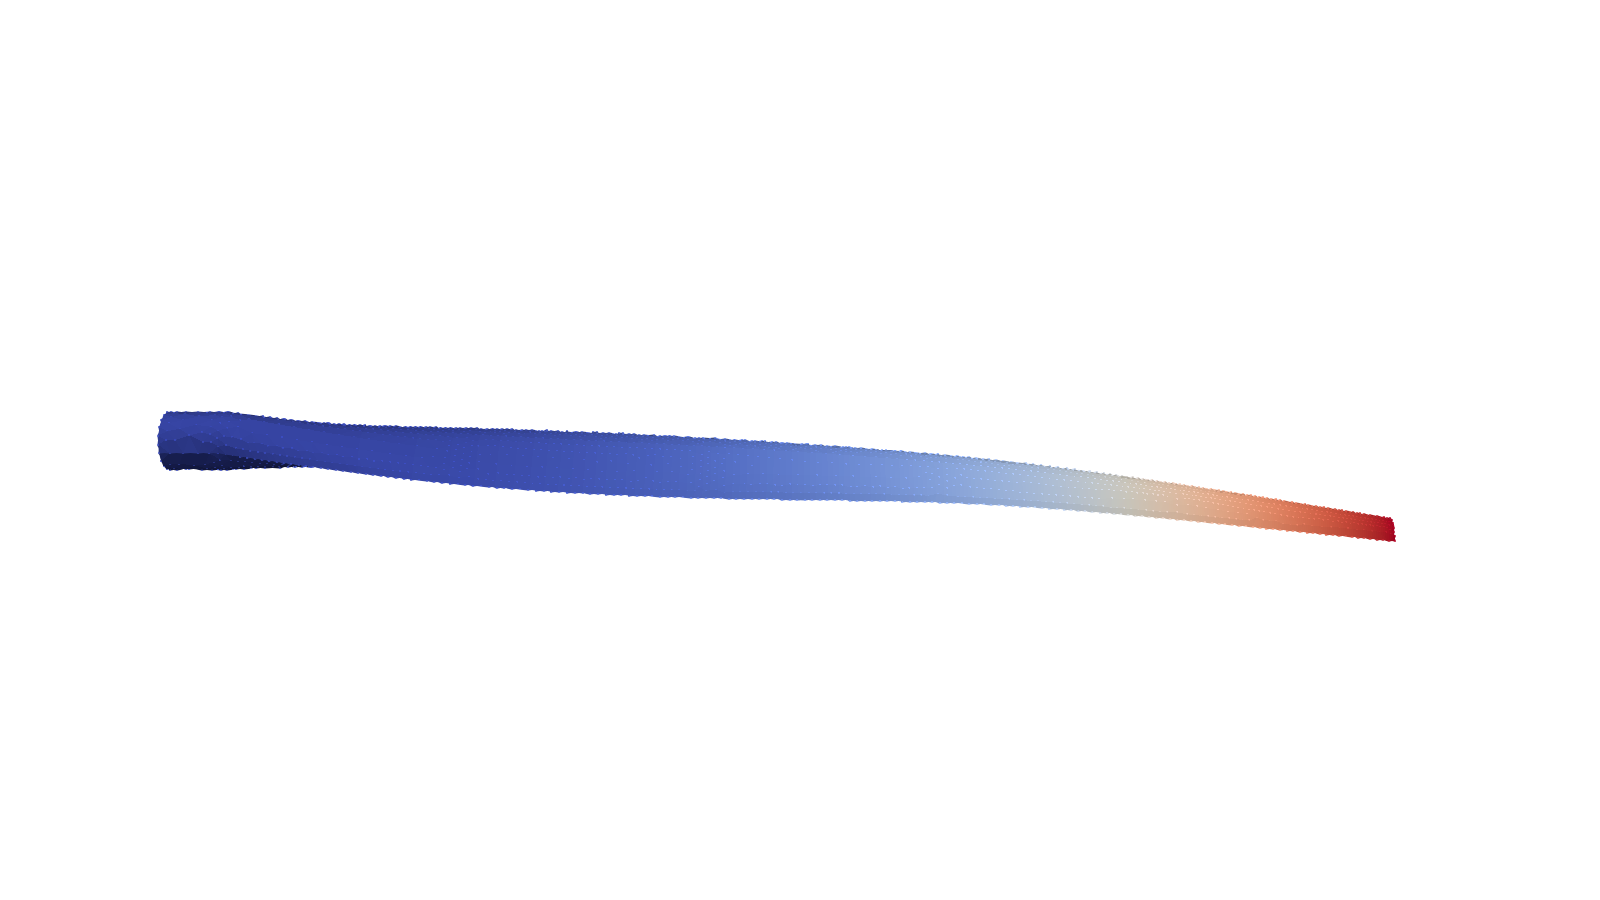
\includegraphics[width=\textwidth]{Figures/WindTurbineBladeModalAnalysisMode1.png}
        \caption{Mode 1: 0.81 Hz}
    \end{subfigure}
    \hfill
    \begin{subfigure}[b]{0.3\textwidth}
        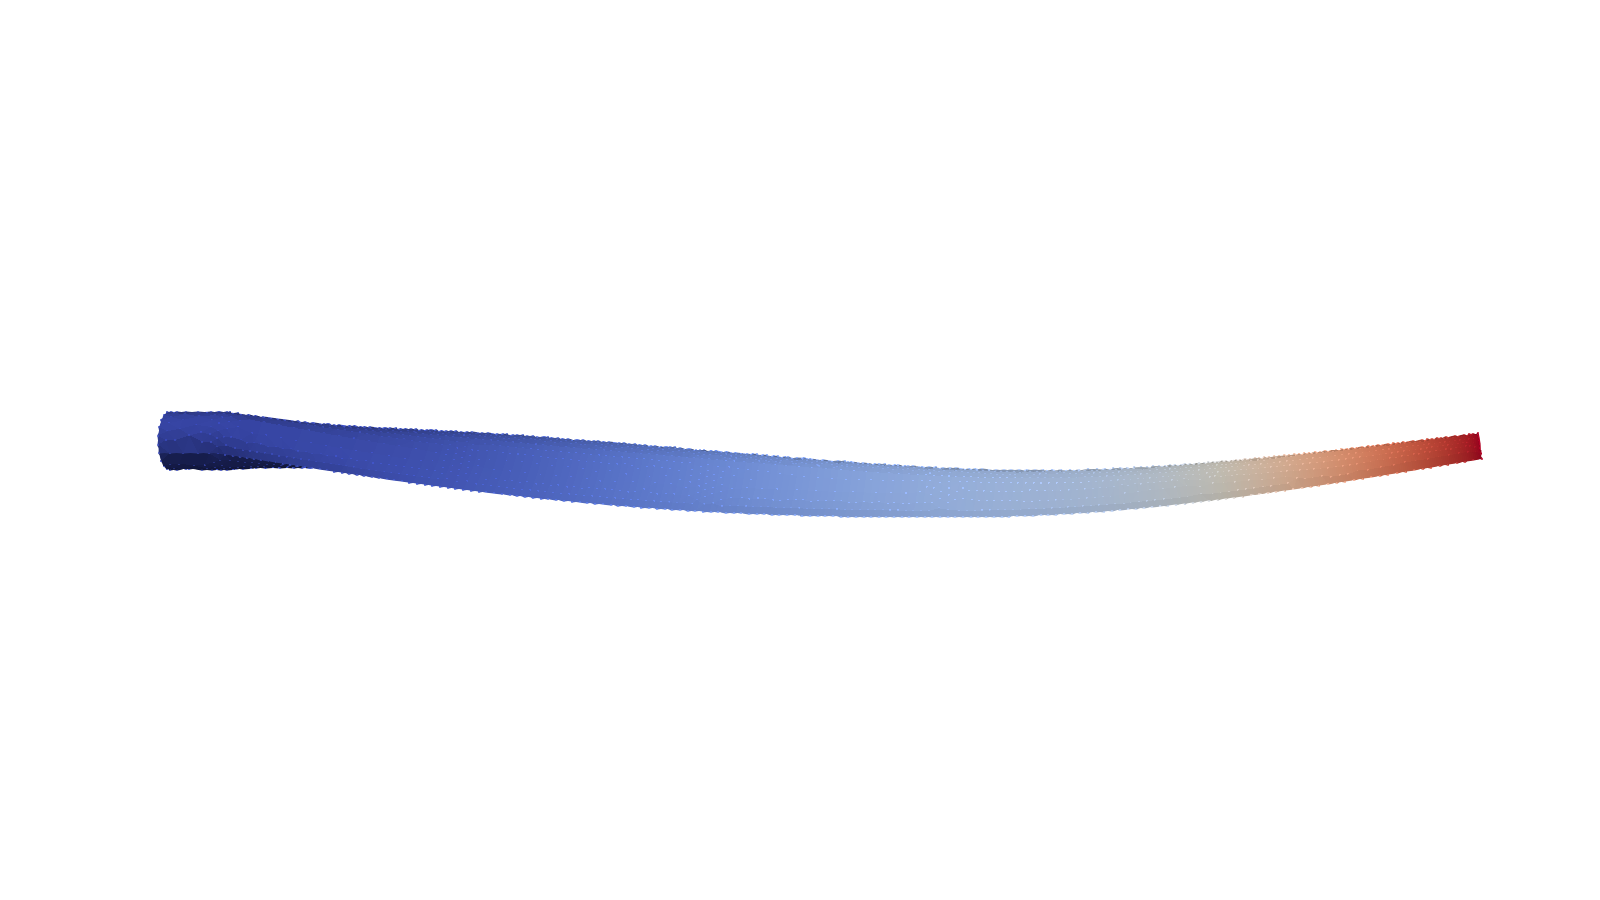
\includegraphics[width=\textwidth]{Figures/WindTurbineBladeModalAnalysisMode2.png}
        \caption{Mode 2: 1.90 Hz}
    \end{subfigure}
    \hfill
    \begin{subfigure}[b]{0.3\textwidth}
        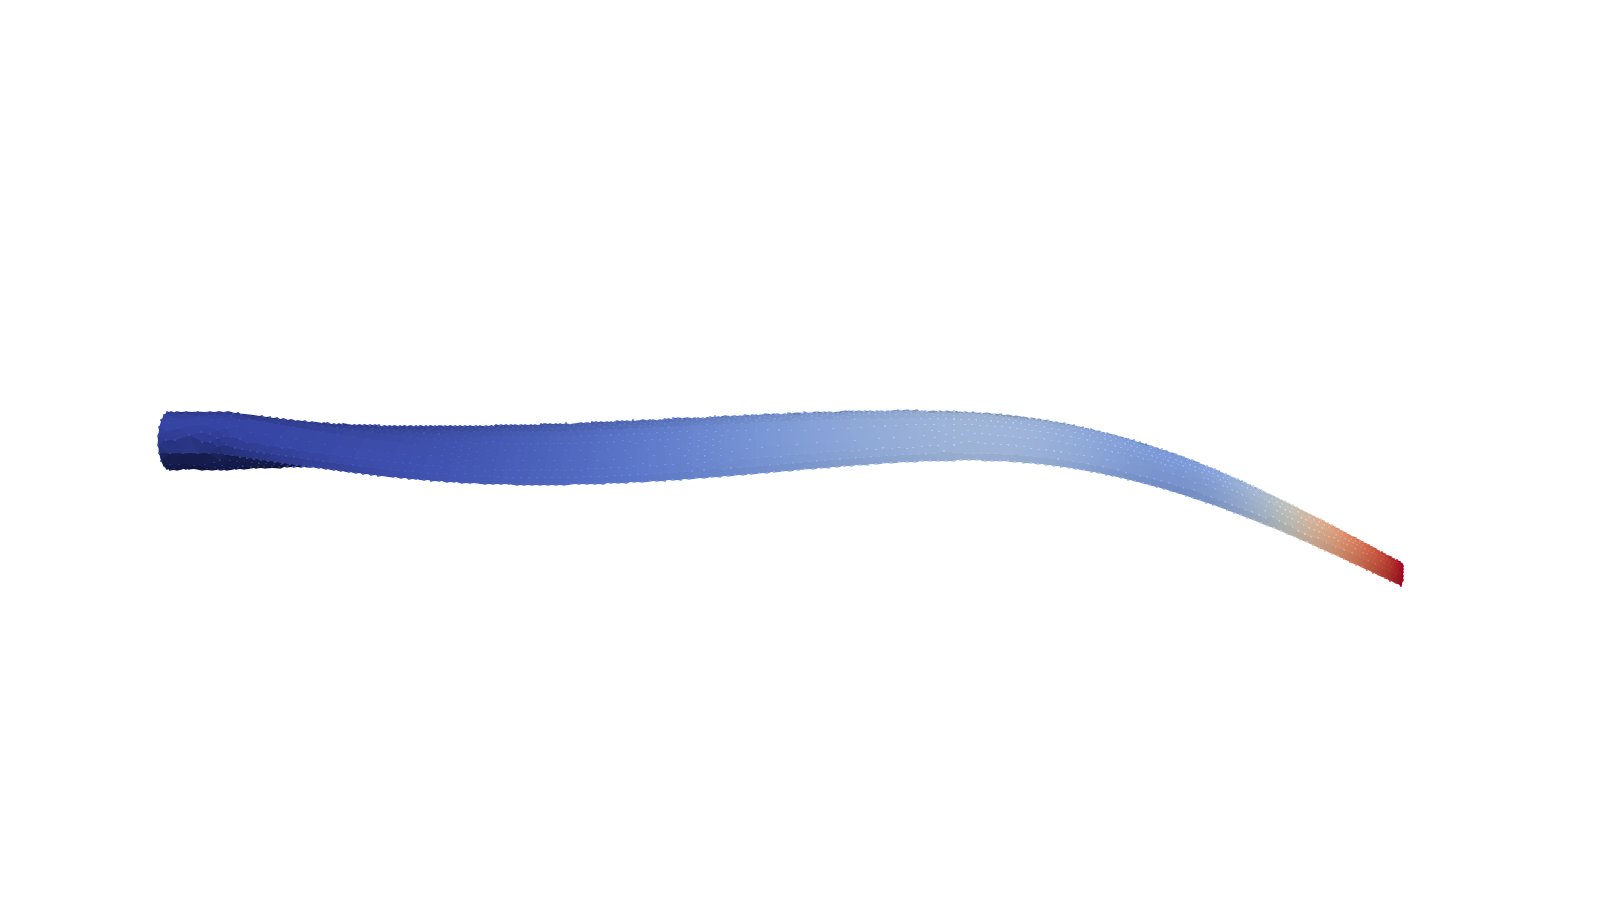
\includegraphics[width=\textwidth]{Figures/WindTurbineBladeModalAnalysisMode3.png}
        \caption{Mode 3: 2.51 Hz}
    \end{subfigure}
    
    \vspace{1em}
    
    \begin{subfigure}[b]{0.3\textwidth}
        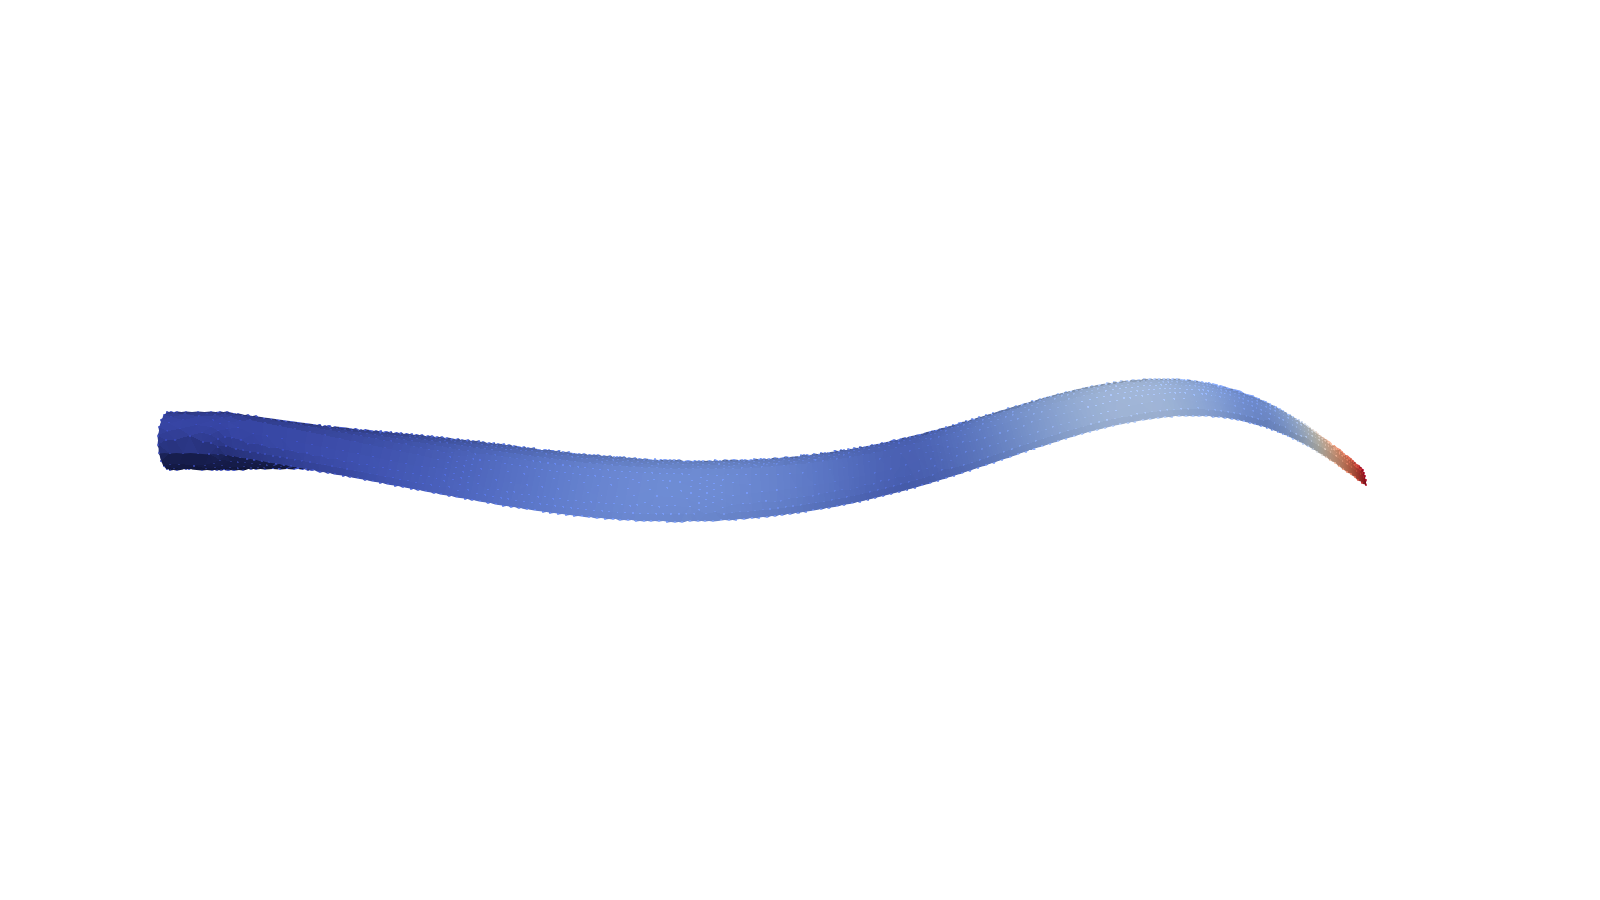
\includegraphics[width=\textwidth]{Figures/WindTurbineBladeModalAnalysisMode4.png}
        \caption{Mode 4: 5.37 Hz}
    \end{subfigure}
    \hfill
    \begin{subfigure}[b]{0.3\textwidth}
        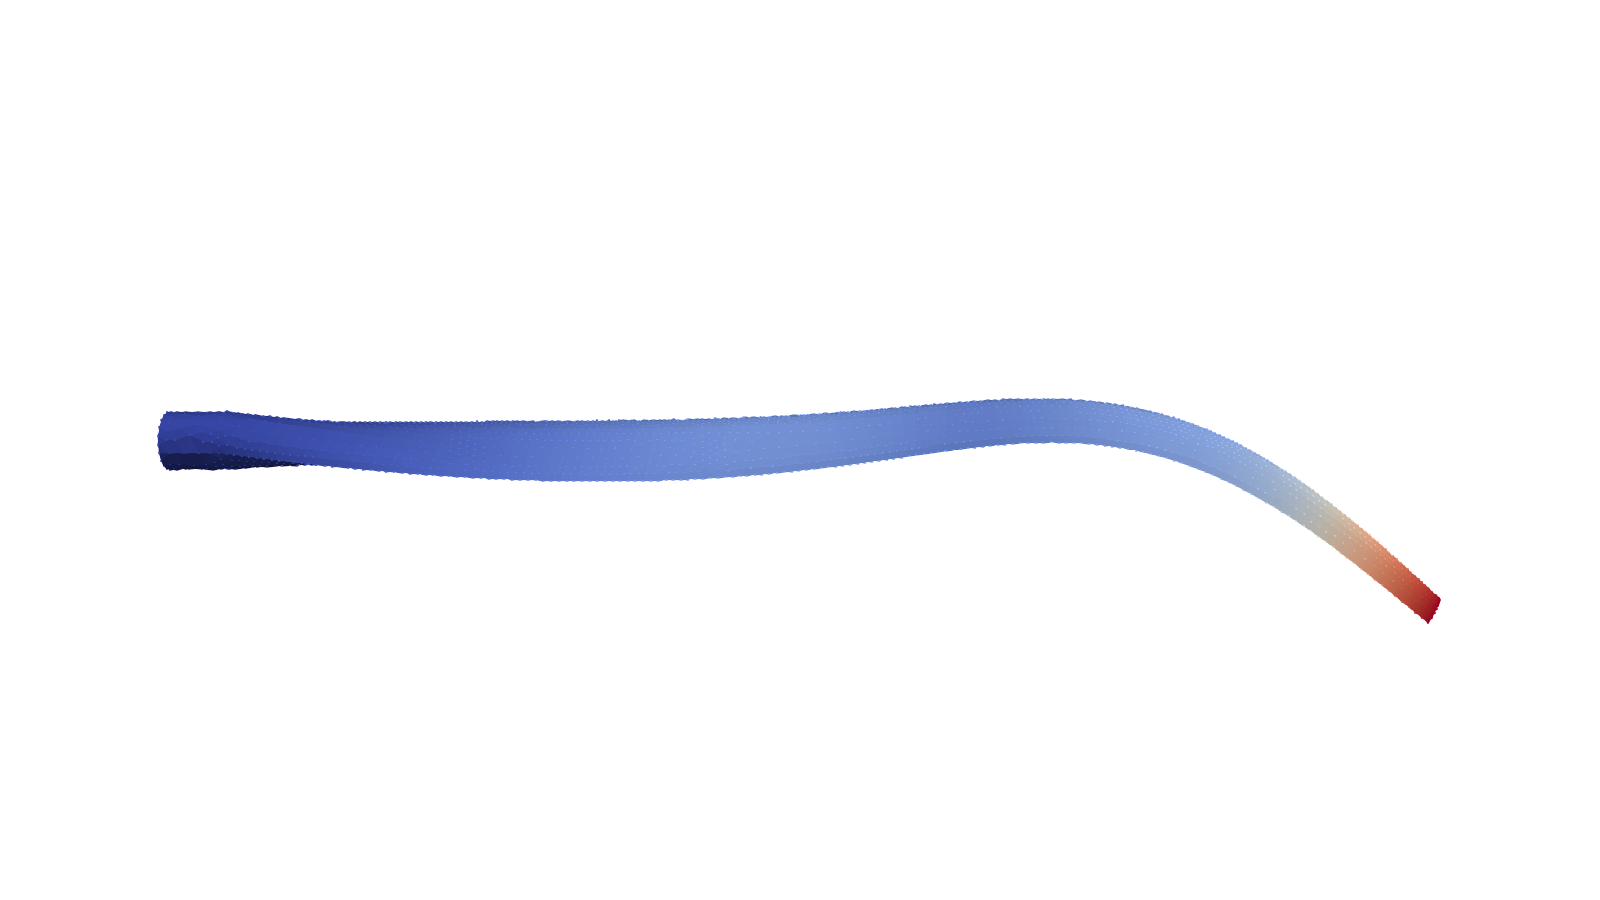
\includegraphics[width=\textwidth]{Figures/WindTurbineBladeModalAnalysisMode5.png}
        \caption{Mode 5: 6.21 Hz}
    \end{subfigure}
    \hfill
    \begin{subfigure}[b]{0.3\textwidth}
        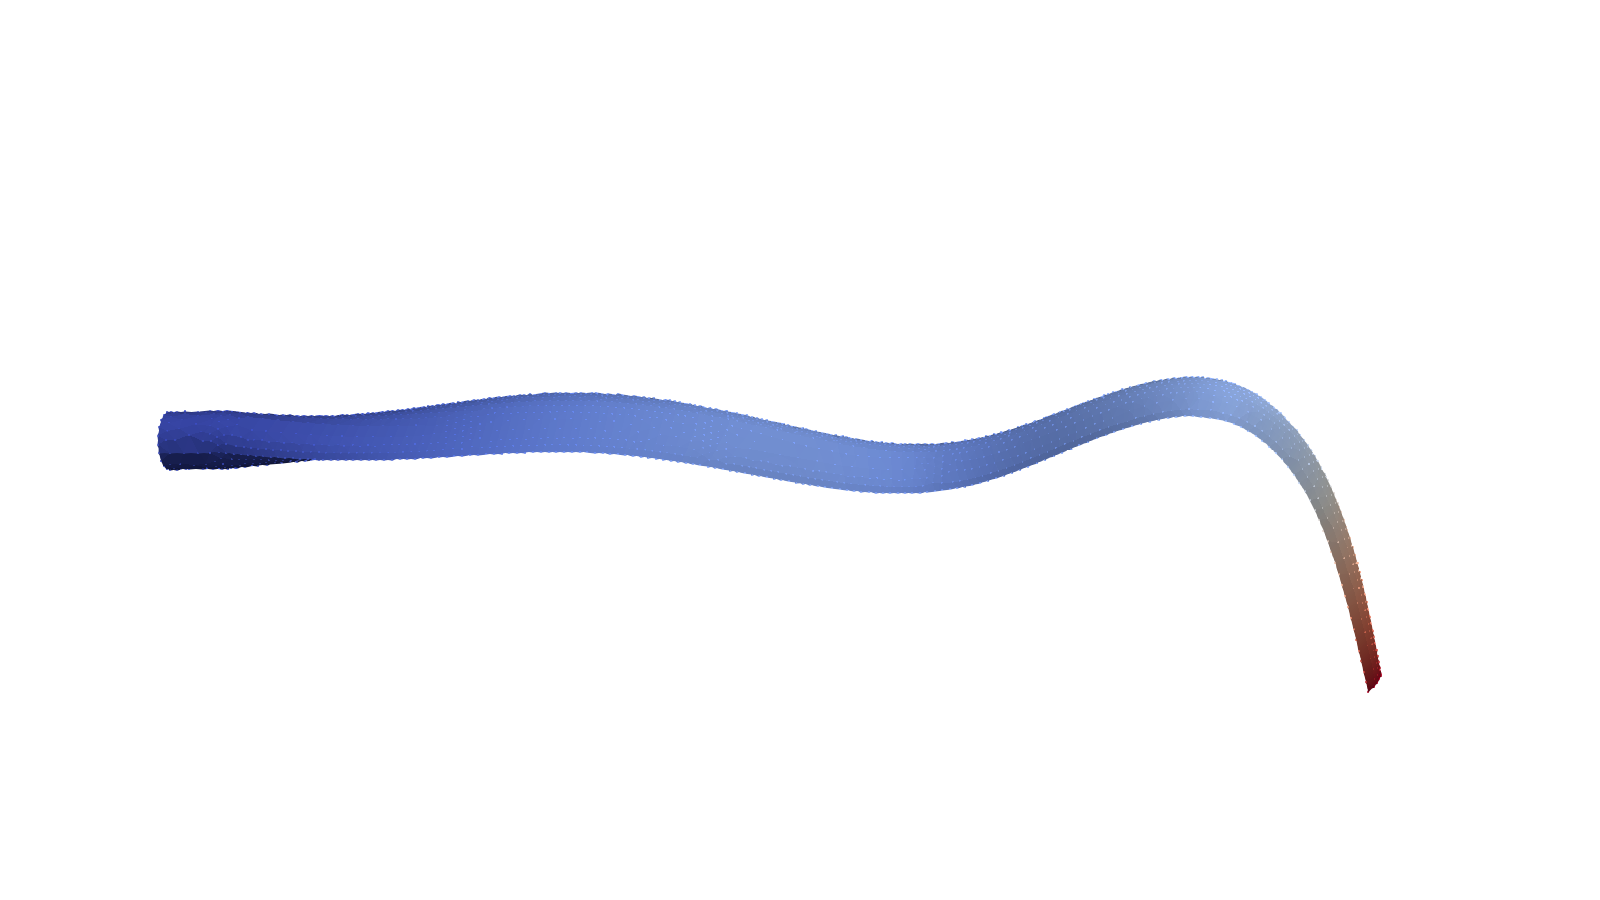
\includegraphics[width=\textwidth]{Figures/WindTurbineBladeModalAnalysisMode6.png}
        \caption{Mode 6: 9.41 Hz}
    \end{subfigure}

    \caption{
    First six vibration modes of the wind turbine blade obtained from free vibration analysis using linear elasticity. The modes are ordered by increasing natural frequency, ranging from 0.81 Hz to 9.41 Hz. The shapes reflect dominant deformation patterns, including bending and torsional behavior, and illustrate the concentration of dynamic energy in a small number of low-frequency modes.
    }
    \label{fig:blade_modes}
\end{figure}


Although the full-order model contains \( N = 17\,683 \) degrees of freedom, the blade's dynamic response is largely governed by a small number of low-frequency modes. This low-dimensional behavior supports the rationale behind projection-based reduction.

While modal analysis is not used directly in this thesis as a solver, it exemplifies the idea of restricting the dynamics to a low-dimensional subspace spanned by physically meaningful basis functions. It also motivates the need for more flexible, data-driven basis construction techniques, such as proper orthogonal decomposition, for problems where linearity, symmetry, or time-invariance do not hold.

\vspace{0.5em}
\textit{See, for example,}~\cite{craig2006fundamentals, meirovitch1975elements, kerschen2005method} \textit{for classical and modern treatments of modal analysis in structural dynamics.}

\section{Proper orthogonal decomposition}

Proper orthogonal decomposition (POD) constructs a low-dimensional linear subspace that best approximates a family of high-dimensional solution snapshots in the least-squares sense.  
Unlike classical modal analysis, POD is data-driven and makes no assumptions about linearity, symmetry, or time-invariance.

Let the system's behavior be governed by underlying equations (often partial differential equations) dependent on spatial coordinates $\mathbf{x} \in \Omega$, time $t \in [0, T]$, and a set of parameters $\boldsymbol{\mu} \in \mathcal{D} \subset \mathbb{R}^p$. The application of a suitable spatial discretization method (e.g., Finite Element, Finite Volume, Finite Difference) to these equations yields the high-fidelity solution, represented by a time- and parameter-dependent state vector $\mathbf{u} \in \mathbb{R}^N$, where $N$ is the number of degrees of freedom.

A specific instance of this discrete state vector at time $t$ and for parameter configuration $\boldsymbol{\mu}$ is denoted as:
\begin{equation}
\mathbf{u}(t, \boldsymbol{\mu}) \in \mathbb{R}^N
\end{equation}
This vector represents the high-dimensional state of the system within the chosen discretization.

For POD, solution snapshots are collected at selected discrete time instances $t_k \in \{t_1, t_2, \dots, t_{N_t}\} \subset [0, T]$ and for various parameter samples $\boldsymbol{\mu}_j \in \{\boldsymbol{\mu}_1, \boldsymbol{\mu}_2, \dots, \boldsymbol{\mu}_P\} \subset \mathcal{D}$. These snapshots are assembled into the columns of the snapshot matrix $\mathbf{S}$:

\begin{equation}
\label{eq:snapshot_matrix}
\mathbf{S} = 
\begin{bmatrix}
\mathbf{u}(t_1, \boldsymbol{\mu}_1), \mathbf{u}(t_2, \boldsymbol{\mu}_1), \dots, \mathbf{u}(t_{N_t}, \boldsymbol{\mu}_1), \mathbf{u}(t_1, \boldsymbol{\mu}_2), \dots, \mathbf{u}(t_{N_t}, \boldsymbol{\mu}_2), \dots, \mathbf{u}(t_1, \boldsymbol{\mu}_P), \dots, \mathbf{u}(t_{N_t}, \boldsymbol{\mu}_P)
\end{bmatrix}
\in \mathbb{R}^{N \times N_s},
\end{equation}
where $N_s = N_t \cdot P$ is the total number of snapshots or samples, $N_t$ is the number of time instances sampled per parameter, and $P$ is the number of parameter samples.

\paragraph{POD basis.}
Given the snapshot matrix $\mathbf{S} \in \mathbb{R}^{N \times N_s}$, the objective of POD is to find an orthonormal matrix $\boldsymbol{\Phi} \in \mathbb{R}^{N \times n}$, whose columns span the $n$-dimensional subspace that minimizes the Frobenius‐norm projection error:
\begin{equation}
\label{eq:pod_opt}
\min_{\boldsymbol{\Phi}^{\!T}\boldsymbol{\Phi}=\mathbf{I}_n}
\;\bigl\|\,\mathbf{S} - \boldsymbol{\Phi}\boldsymbol{\Phi}^{\!T}\mathbf{S}\bigr\|_{F}^{2}.
\end{equation}
Here, $\mathbf{I}_n$ is the $n \times n$ identity matrix, and $\boldsymbol{\Phi}\boldsymbol{\Phi}^{\!T}$ represents the orthogonal projector onto the subspace spanned by the columns of $\boldsymbol{\Phi}$. The solution to this optimization problem \eqref{eq:pod_opt} is obtained via the SVD of the snapshot matrix. Considering the thin SVD,
\begin{equation}
\mathbf{S}= \mathbf{U}\boldsymbol{\Sigma}\mathbf{V}^{\!T},
\end{equation}
where $\mathbf{U} \in \mathbb{R}^{N \times r}$ has orthonormal columns (left singular vectors), $\mathbf{V} \in \mathbb{R}^{N_s \times r}$ has orthonormal columns (right singular vectors), $r = \operatorname{rank}(\mathbf{S})$, and $\boldsymbol{\Sigma}=\operatorname{diag}(\sigma_1,\dots,\sigma_r) \in \mathbb{R}^{r \times r}$ contains the positive singular values ordered non-increasingly ($\sigma_1 \ge \sigma_2 \ge \dots \ge \sigma_r > 0$). The optimal rank-$n$ POD basis ($n \le r$) consists of the first $n$ left singular vectors:
\begin{equation}
\boldsymbol{\Phi}= \mathbf{U}_{[:,1:n]}.
\end{equation}

\paragraph{Energy criterion.}
A common heuristic for selecting the basis dimension $n$ involves monitoring the cumulative energy captured by the retained singular values. The \emph{squared POD energy loss}, or fraction of unexplained variance, is defined as:
\begin{equation}
\label{eq:pod_energy_loss}
\epsilon^{2}(n)
\;=\;
1 - \frac{\displaystyle\sum_{i=1}^{n}\sigma_i^{\,2}}
         {\displaystyle\sum_{j=1}^{r}\sigma_j^{\,2}},
\qquad 0 \le \epsilon^{2}(n) \le 1,
\end{equation}
This quantity $\epsilon^2(n)$ represents the fraction of energy discarded by the rank-$n$ approximation. Intuitively, it quantifies the proportion of the system’s dynamic energy not captured by the reduced basis.

It is equivalent to the squared relative reconstruction error of the snapshot matrix in the Frobenius norm:
\begin{equation}
\epsilon^2(n) = \frac{\|\mathbf{S} - \boldsymbol{\Phi}\boldsymbol{\Phi}^{\!T}\mathbf{S}\|_F^2}{\|\mathbf{S}\|_F^2}.
\end{equation}
Consequently, $\epsilon(n)$ is the relative Frobenius error associated with approximating $\mathbf{S}$ by its projection onto the $n$-dimensional POD basis $\boldsymbol{\Phi}$. A desired tolerance $\epsilon_{tol}$ is often set (e.g., $10^{-3}$), and the smallest $n$ is chosen such that $\epsilon(n) \le \epsilon_{tol}$.


\subsection{Projection-based reduced order model via Galerkin projection}

Let $\mathbf{R}(\mathbf{u}(t,\boldsymbol{\mu});\,t,\boldsymbol{\mu}) = \mathbf{0}$ 
denote a general discrete residual arising from a finite element, finite volume, or finite difference discretization, such as the one introduced in Section~\ref{sec:model_problem}. 
Here, $\mathbf{u}(t,\boldsymbol{\mu}) \in \mathbb{R}^N$ is the full-order solution at time $t$ and parameter $\boldsymbol{\mu} \in \mathcal{D}$.

In projection-based model reduction, $\mathbf{u}(t,\boldsymbol{\mu})$ is approximated as
\begin{equation}
\mathbf{u}(t,\boldsymbol{\mu}) \;\approx\; 
\mathbf{\tilde{u}}(t,\boldsymbol{\mu}) 
= \mathbf{u}_{\text{ref}} + \boldsymbol{\Phi}\,\mathbf{q}(t,\boldsymbol{\mu}),
\end{equation}
where $\mathbf{u}_{\text{ref}} \in \mathbb{R}^N$ is a reference state, 
$\boldsymbol{\Phi} \in \mathbb{R}^{N \times n}$ is the reduced basis matrix, 
and $\mathbf{q}(t,\boldsymbol{\mu}) \in \mathbb{R}^n$ are the reduced generalized coordinates. 
The reference $\mathbf{u}_{\text{ref}}$ is often chosen as the mean of the snapshot set or as the initial condition of the system. 
For simplicity, and without loss of generality in the following derivations, 
we take $\mathbf{u}_{\text{ref}} = \mathbf{0}$.  

The encoder–decoder structure of this approximation is illustrated in Figure~\ref{fig:linear_reduction_encoder_decoder}.


\begin{figure}[ht!]
    \centering
    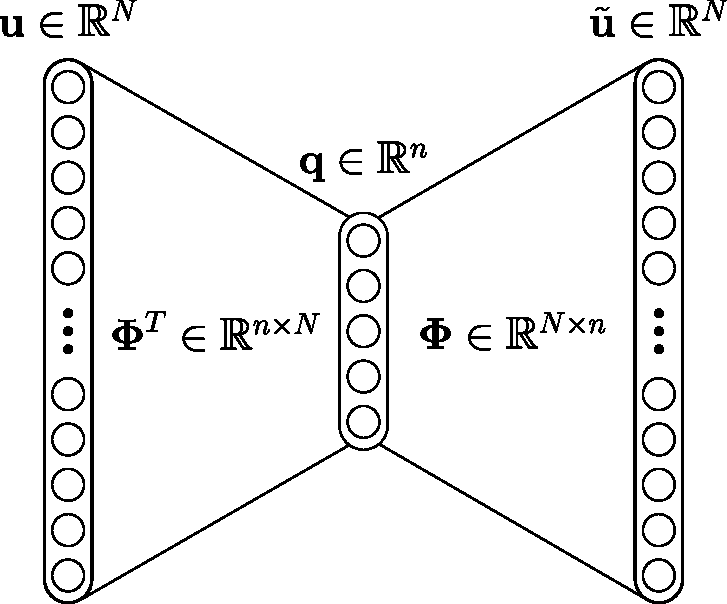
\includegraphics[width=0.5\textwidth]{Figures/linear_prom_encoder_decoder.pdf}
    \caption{
    Schematic representation of the linear subspace reduction and reconstruction process.
    The high-dimensional state \( \mathbf{u} \in \mathbb{R}^N \) is projected onto a low-dimensional subspace via \( \mathbf{q} = \boldsymbol{\Phi}^T \mathbf{u} \), and an approximation \( \tilde{\mathbf{u}} = \boldsymbol{\Phi} \mathbf{q} \) is reconstructed from the reduced coordinates \( \mathbf{q} \in \mathbb{R}^n \).
    }
    \label{fig:linear_reduction_encoder_decoder}
\end{figure}


The Galerkin projection seeks a reduced solution such that the residual is orthogonal to the subspace spanned by \( \boldsymbol{\Phi} \), i.e.,
\begin{equation}
\boldsymbol{\Phi}^{\!T}\,\mathbf{R}\bigl(\boldsymbol{\Phi}\,\mathbf{q}(t,\boldsymbol{\mu});\, t,\boldsymbol{\mu}\bigr) = \mathbf{0},
\label{eq:galerkin_orthogonality}
\end{equation}

\begin{equation}
\mathbf{R}_{r}\bigl(\mathbf{q}(t,\boldsymbol{\mu});\, t,\boldsymbol{\mu}\bigr)
\;:=\;
\boldsymbol{\Phi}^{\!T}\,\mathbf{R}\bigl(\boldsymbol{\Phi}\,\mathbf{q}(t,\boldsymbol{\mu});\, t,\boldsymbol{\mu}\bigr)
\in \mathbb{R}^{n}.
\label{eq:galerkin_reduced_residual}
\end{equation}



In the nonlinear case, the reduced system cannot be solved directly and requires iterative methods. A common approach is Newton’s method (applied to the projected residual), which yields the reduced linear system at each iteration (schematically illustrated in Figure~\ref{fig:galerkin_newton_projection}):
\begin{subequations}
\begin{align}
\mathbf{J}_{r}\bigl(\mathbf{q}^{(k)}(t,\boldsymbol{\mu});\,t,\boldsymbol{\mu}\bigr)\,\delta \mathbf{q}^{(k)} 
&= -\,\mathbf{R}_{r}\bigl(\mathbf{q}^{(k)}(t,\boldsymbol{\mu});\,t,\boldsymbol{\mu}\bigr),
\label{eq:galerkin_newton_linear}\\[0.5em]
\mathbf{q}^{(k+1)}(t,\boldsymbol{\mu}) 
&= \mathbf{q}^{(k)}(t,\boldsymbol{\mu}) + \delta \mathbf{q}^{(k)}.
\label{eq:galerkin_newton_update}
\end{align}
\end{subequations}


\begin{figure}[ht!]
    \centering
    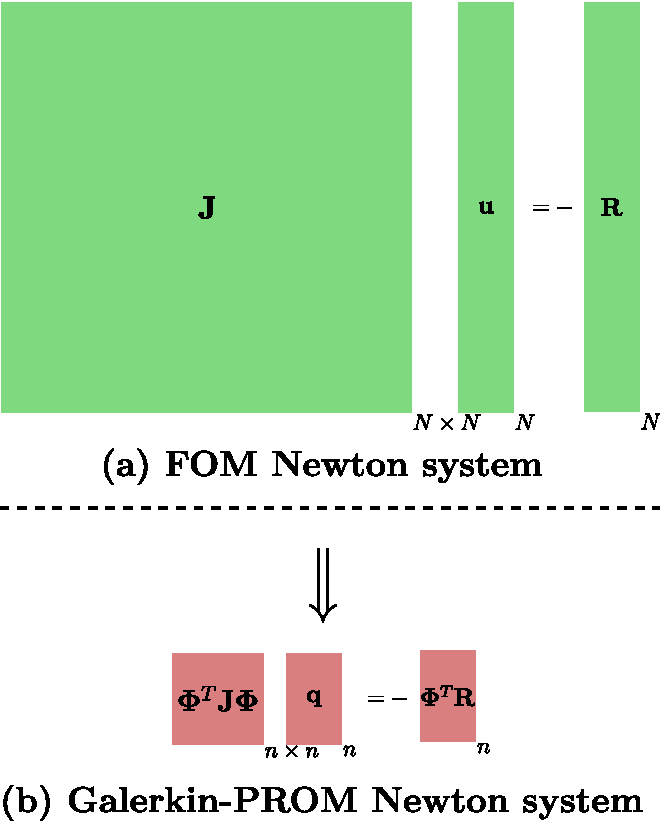
\includegraphics[width=0.52\textwidth]{Figures/SystemReduction2.pdf}
    \caption{
    Visual comparison of Newton systems before and after Galerkin projection.
    \textbf{(a)} Full-order model (FOM) Newton system: the nonlinear system is defined over the high-dimensional space \( \mathbb{R}^N \), involving the full residual \( \mathbf{R} \) and Jacobian \( \mathbf{J} \).
    \textbf{(b)} Galerkin-PROM system: projection via the reduced basis \( \boldsymbol{\Phi} \) yields a low-dimensional system in terms of reduced coordinates \( \mathbf{q} \in \mathbb{R}^n \).
    }
    \label{fig:galerkin_newton_projection}
\end{figure}


where \( \delta \mathbf{q} \in \mathbb{R}^n \) is the correction to the reduced state iterate, and the reduced Jacobian \( \mathbf{J}_{r} \) (evaluated at the current iterate \( \mathbf{q}(t, \boldsymbol{\mu}) \)) is given by
\begin{equation}
\label{eq:reduced_jacobian}
\mathbf{J}_{r}\bigl(\mathbf{q}(t,\boldsymbol{\mu});\,t,\boldsymbol{\mu}\bigr) 
= \boldsymbol{\Phi}^{\!T}\,
\mathbf{J}\bigl(\boldsymbol{\Phi}\,\mathbf{q}(t,\boldsymbol{\mu});\,t,\boldsymbol{\mu}\bigr)\,
\boldsymbol{\Phi}
\;\in\; \mathbb{R}^{n \times n}.
\end{equation}
Here, \( \mathbf{J}(\mathbf{u};\,t,\boldsymbol{\mu}) \in \mathbb{R}^{N \times N} \) is the full-order Jacobian matrix, defined as the derivative of the full-order residual with respect to the full-order state:
\begin{equation}
\label{eq:full_jacobian_def}
\mathbf{J}\bigl(\mathbf{u}(t,\boldsymbol{\mu});\,t,\boldsymbol{\mu}\bigr) 
:= \frac{\partial \mathbf{R}\bigl(\mathbf{u}(t,\boldsymbol{\mu});\,t,\boldsymbol{\mu}\bigr)}{\partial \mathbf{u}}.
\end{equation}

In Equation~\eqref{eq:reduced_jacobian}, the full-order Jacobian \( \mathbf{J} \) is evaluated at the state corresponding to the current reduced iterate, i.e., \( \mathbf{u}(t, \boldsymbol{\mu}) = \boldsymbol{\Phi}\mathbf{q}(t, \boldsymbol{\mu}) \).

While Galerkin projection is optimal when the full-order Jacobian 
\(\mathbf{J}\bigl(\mathbf{u}(t,\boldsymbol{\mu});\,t,\boldsymbol{\mu}\bigr)\) 
is symmetric and positive-definite, it may perform poorly for convection-dominated problems, as there is no guarantee of optimality. A more general treatment of these issues is provided in Section~\ref{subsec:galerkin_lspg_comparison} and Chapter~\ref{chap:article1}, where a Petrov--Galerkin formulation is introduced.

\subsection{POD-Galerkin PROM for the wind turbine blade}

To demonstrate the capabilities of POD for nonlinear dynamics and overcome the limitations of linear modal analysis, a projection-based reduced-order model is developed for the turbine blade. This problem, governed by second-order structural dynamics, is representative of a \emph{parabolic-type} system, characterized by smooth time evolution and symmetric positive-definite operators. The PROM is constructed using snapshots generated by a high-fidelity simulation (FOM).

\paragraph{Full-order model.}
The geometry, illustrated in Figure~\ref{fig:blade_geometry}, corresponds to a utility-scale wind turbine blade approximately 43.2~m in length, with a maximum chord of 3.1~m and a root diameter of around 2~m. The structure is modeled as a solid, homogeneous, and isotropic body to simplify internal detail while retaining global flexibility. The material properties are defined as
\begin{equation}
\rho = 108.48\;\text{kg\,m}^{-3}, 
\qquad   
E   = 2.333\;\text{GPa},
\qquad   
\nu = 0.29.
\end{equation}
The structural response is computed via dynamic analysis using Total Lagrangian solid elements and a compressible Neo-Hookean hyperelastic constitutive law. Large displacements and geometric nonlinearity are fully accounted for. The blade is clamped at the root by homogeneous Dirichlet conditions, no damping is included, and time integration is performed using the implicit Newmark average-acceleration method. The resulting FOM comprises $13\,488$ elements and $17\,683$ degrees of freedom.

\begin{figure}[ht!]
    \centering
    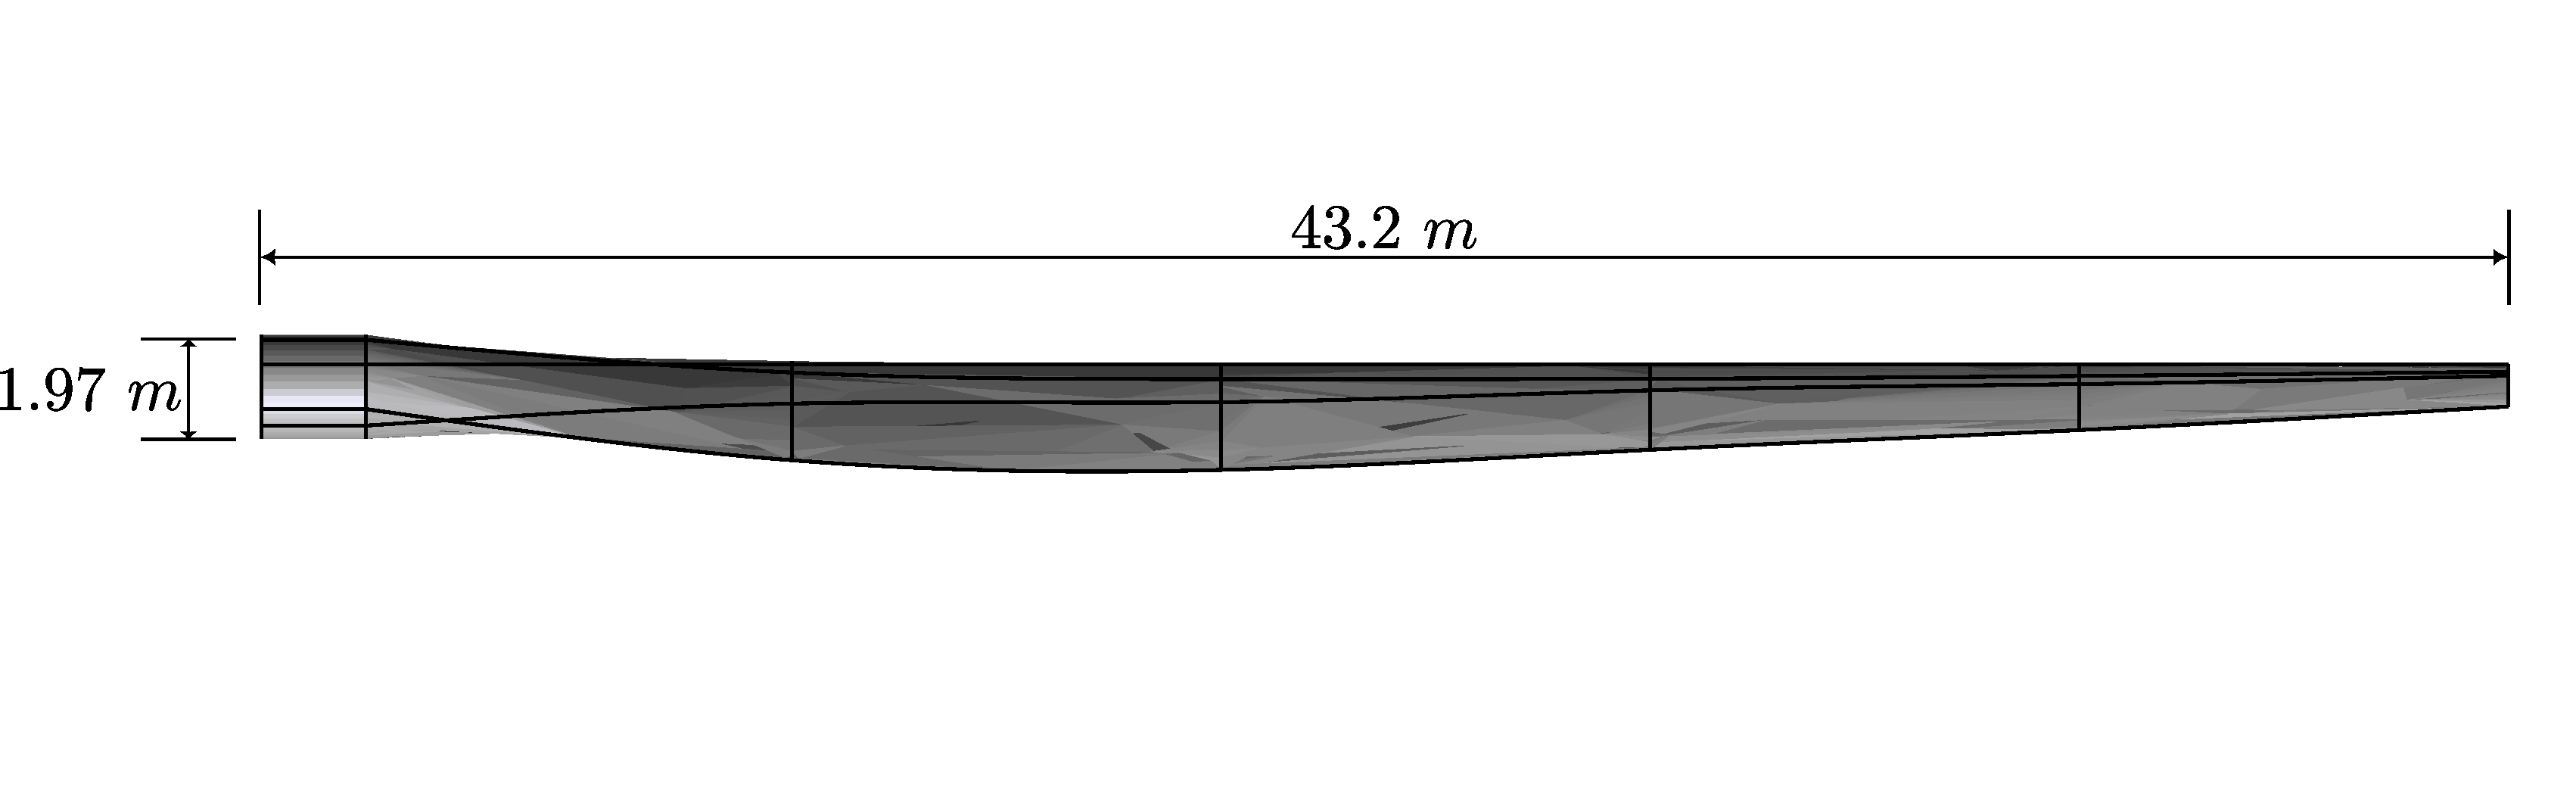
\includegraphics[width=0.85\textwidth]{Figures/WindTurbineBladeGeometry.pdf}
    \caption{
        Geometry and dimensions of the blade under study.
    }
    \label{fig:blade_geometry}
\end{figure}



\paragraph{Transient surface loading.}
Four smooth pressure pulses are imposed on the suction side, each lasting \(T_p = 2\,\text{s}\).  
The spatial and temporal variation is defined as
\begin{equation}
f(x,t) = A_i\, \sin^2\left( \dfrac{\pi (t - t_i)}{T_p} \right) \left( \frac{x}{L} \right)^2, \qquad t \in [t_i, t_i + T_p],
\end{equation}
where \(x\) denotes the axial position along the blade length. The amplitudes are specified as \(A = [500, 400, 600, 300]\,\text{Pa}\) for the training case and \(A = [500, 350, 650, 250]\,\text{Pa}\) for testing.

\begin{figure}[ht!]
    \centering
    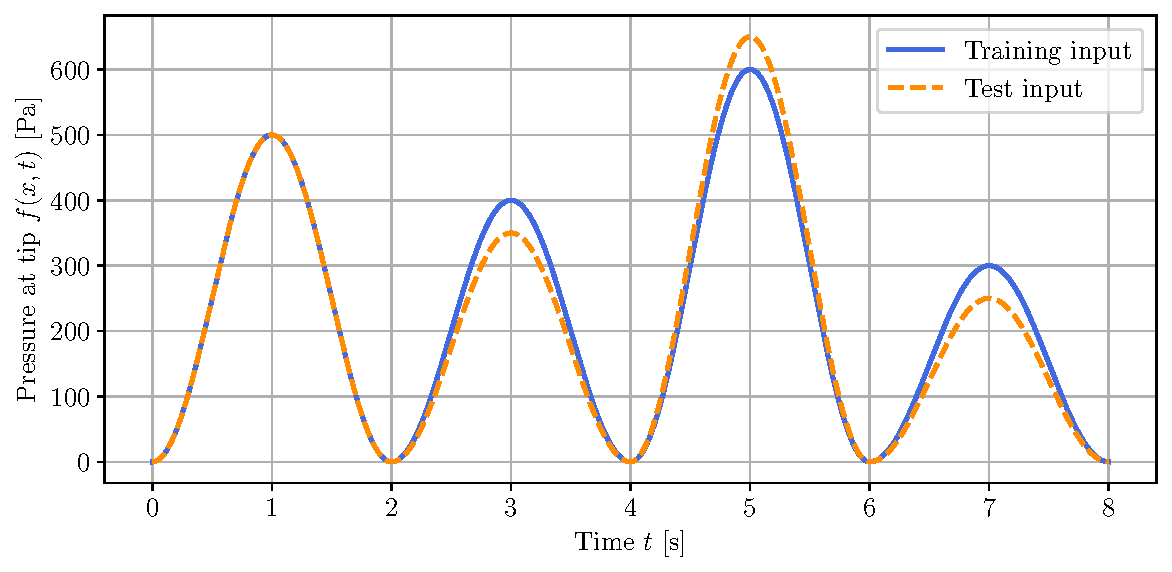
\includegraphics[width=0.85\textwidth]{Figures/training_vs_test_pressure_tip_pa.pdf}
    \caption{
        Time evolution of the pressure input at the blade tip for both training and test cases. 
        Each case consists of four localized pulses with smooth temporal profiles and slight amplitude variations used to evaluate generalization.
    }
    \label{fig:training_test_pulses}
\end{figure}

These loads drive the blade tip through displacements of approximately \(4\,\text{m}\), which is sufficient to trigger pronounced nonlinear effects while remaining within physically plausible bounds for large-scale blades (see Figure~\ref{fig:training_test_pulses}).


\paragraph{Snapshot collection and POD.}
The simulation is performed over a time interval \(t \in [0, 8]\,\text{s}\), using a constant time step \(\Delta t = 0.01\,\text{s}\). A total of 800 solution snapshots are collected during the training run and arranged into the snapshot matrix \(\mathbf{S} \in \mathbb{R}^{N \times N_s}\), where each column corresponds to a full-order solution vector at a given time.  
The singular values of \(\mathbf{S}\) decay rapidly (Figure~\ref{fig:svd_decay}), and the first \(n\) modes capture nearly all of the dynamic energy, enabling an efficient low-rank representation of the system evolution.

\begin{figure}[ht!]
    \centering
    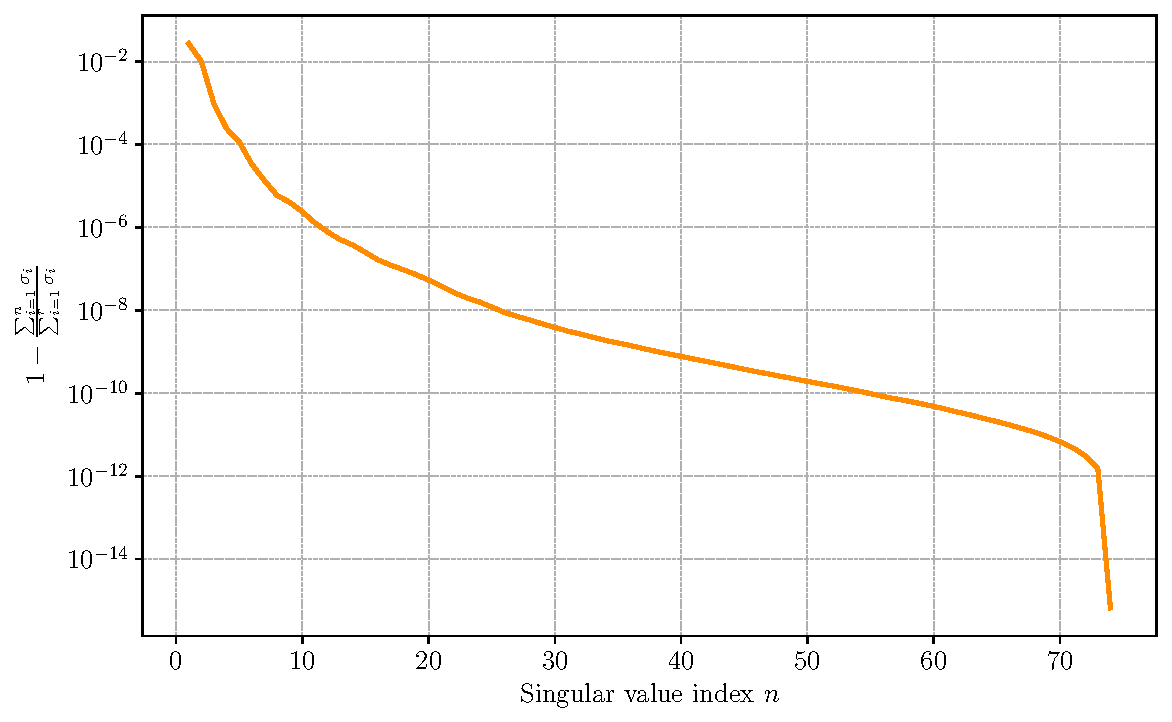
\includegraphics[width=0.65\textwidth]{Figures/svd_relative_loss_linear.pdf}
    \caption{
    Decay of the singular value energy fraction of the singular values of the snapshot matrix. The rapid decay reflects the compressibility of the solution manifold and justifies the use of a low-rank approximation.
    }
    \label{fig:svd_decay}
\end{figure}



\paragraph{POD basis and PROM assembly.}
The leading POD modes (Figure~\ref{fig:blade_pod_modes}) furnish the trial basis \(\boldsymbol{\Phi}\).  
Galerkin projection of the discrete residual yields the POD PROM.  
Accuracy is assessed against the perturbed test pulses.

\begin{figure}[ht!]
    \centering
    \begin{subfigure}[b]{0.3\textwidth}
        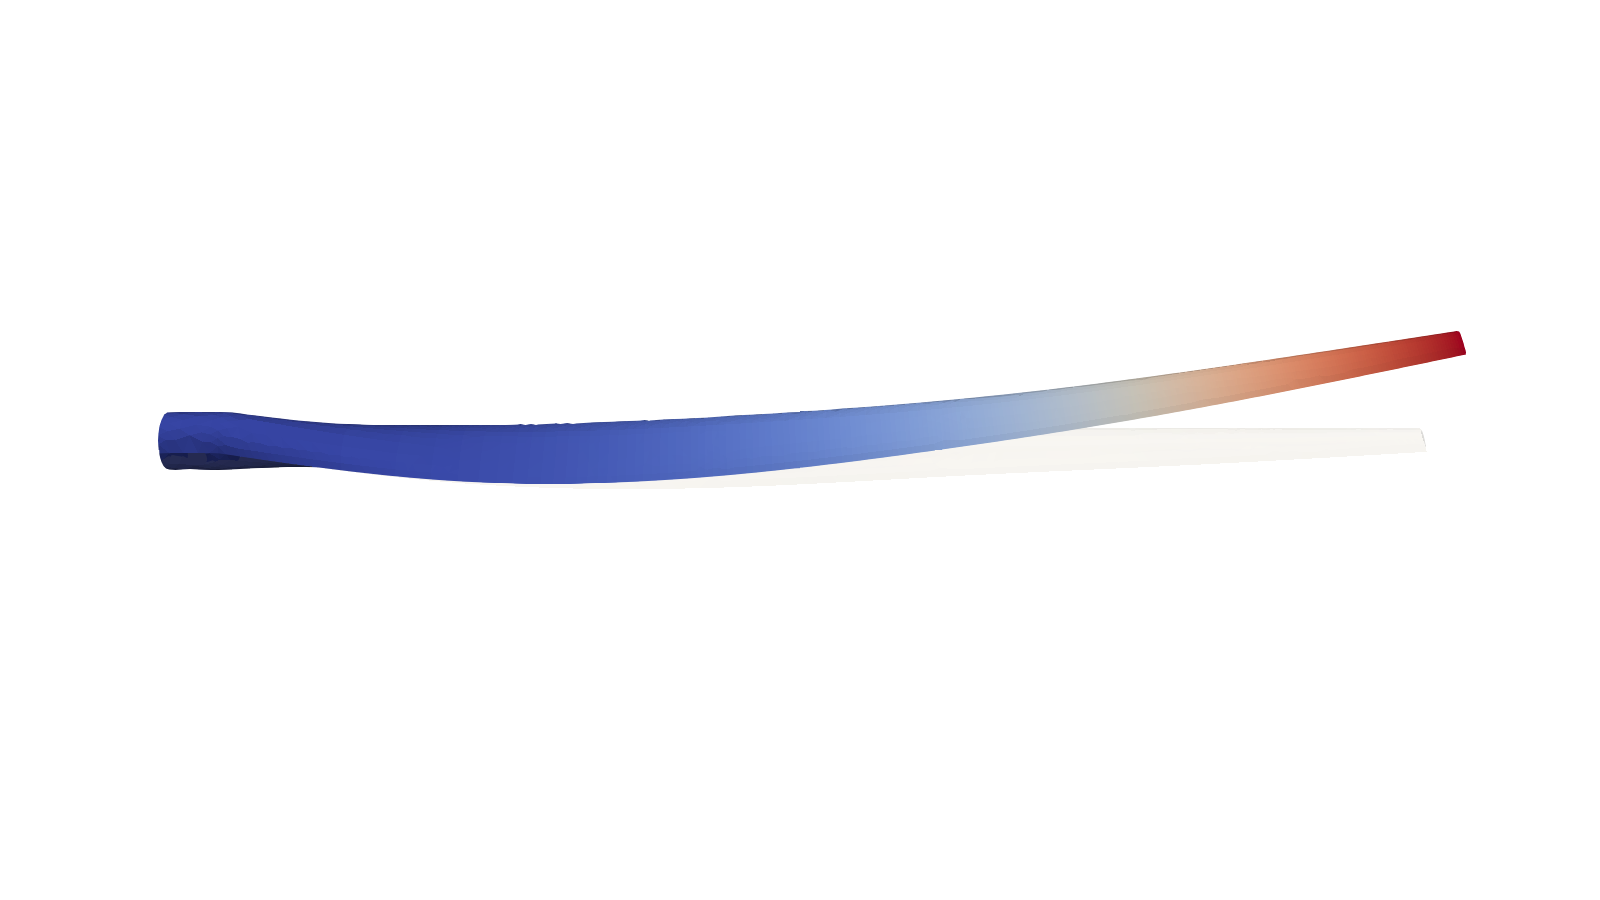
\includegraphics[width=\textwidth]{Figures/WindTurbineBladePODMode1.png}
        \caption{Mode 1}
    \end{subfigure}
    \hfill
    \begin{subfigure}[b]{0.3\textwidth}
        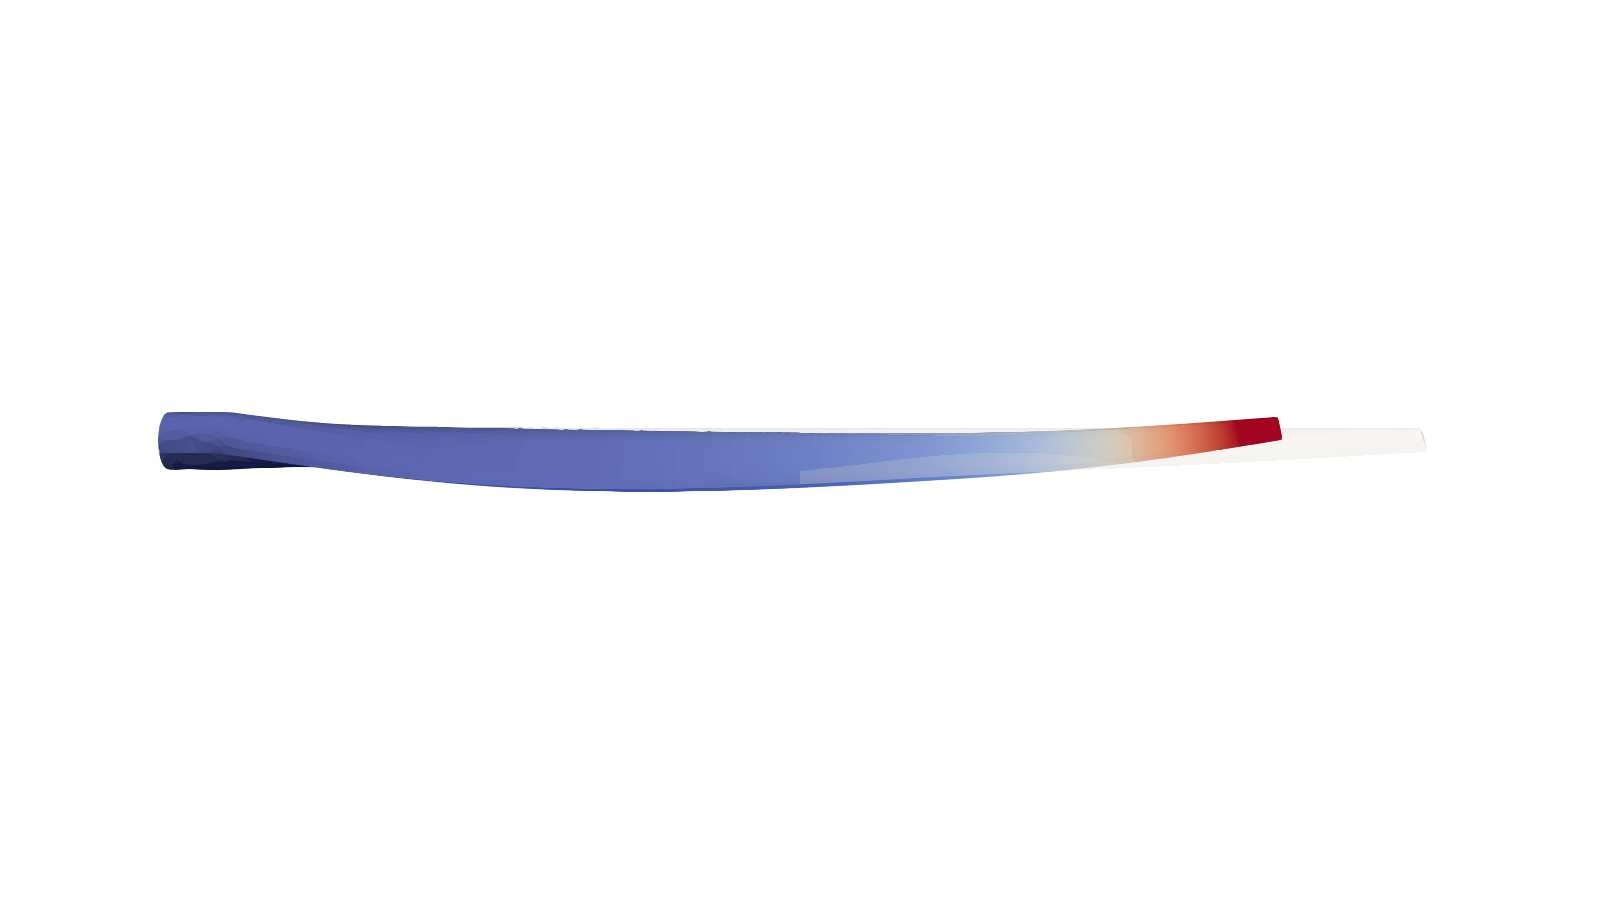
\includegraphics[width=\textwidth]{Figures/WindTurbineBladePODMode2.png}
        \caption{Mode 2}
    \end{subfigure}
    \hfill
    \begin{subfigure}[b]{0.3\textwidth}
        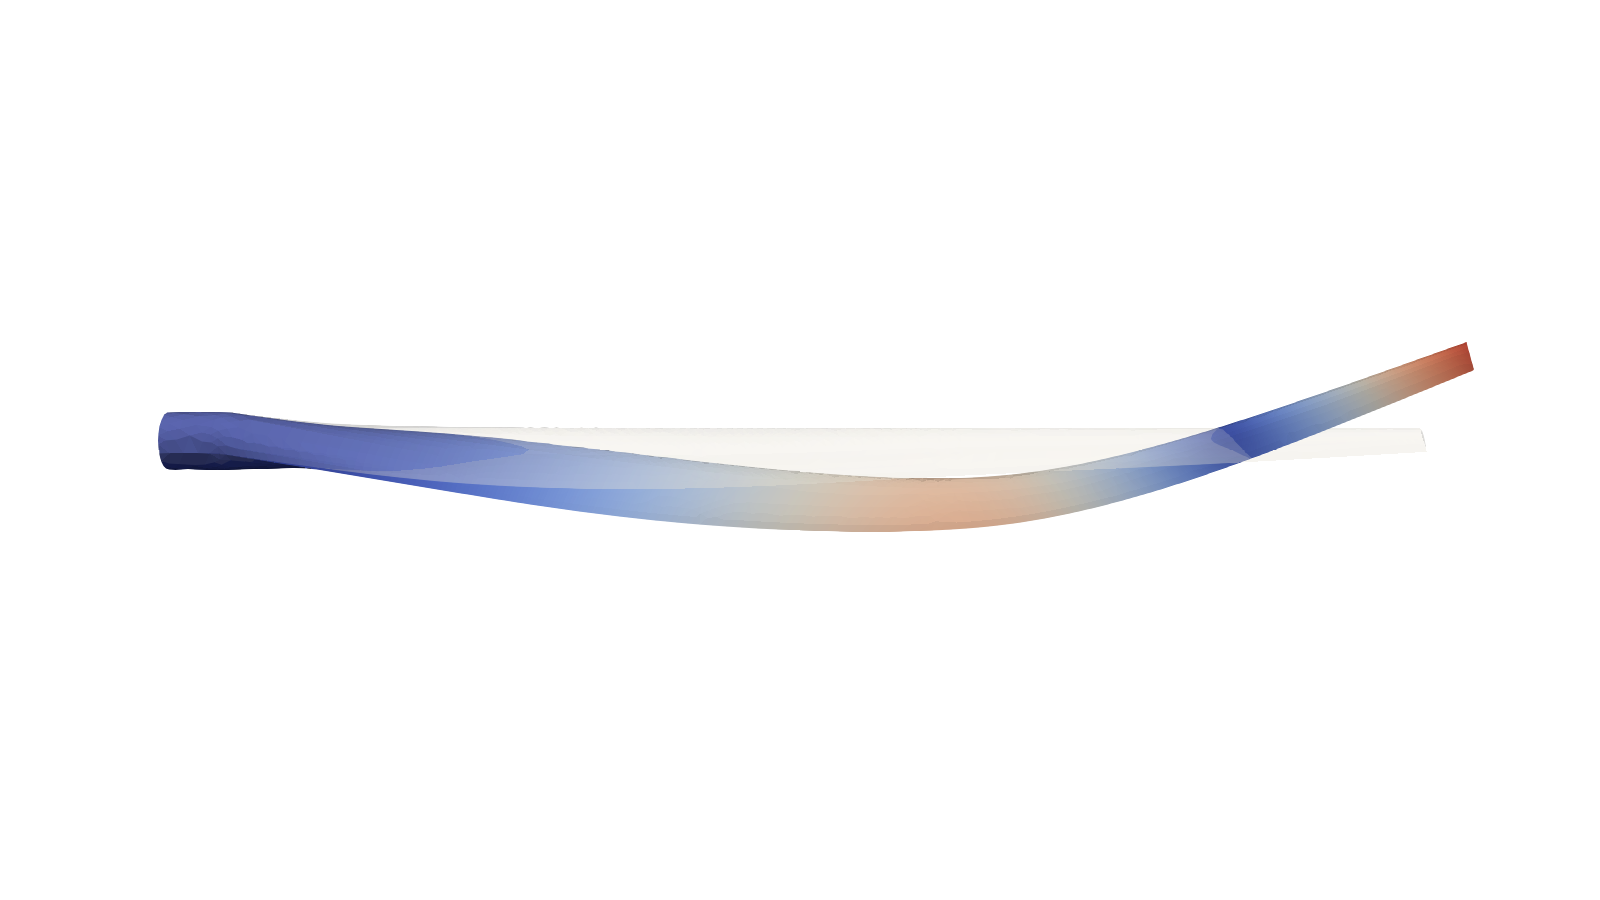
\includegraphics[width=\textwidth]{Figures/WindTurbineBladePODMode3.png}
        \caption{Mode 3}
    \end{subfigure}
    
    \vspace{1em}
    
    \begin{subfigure}[b]{0.3\textwidth}
        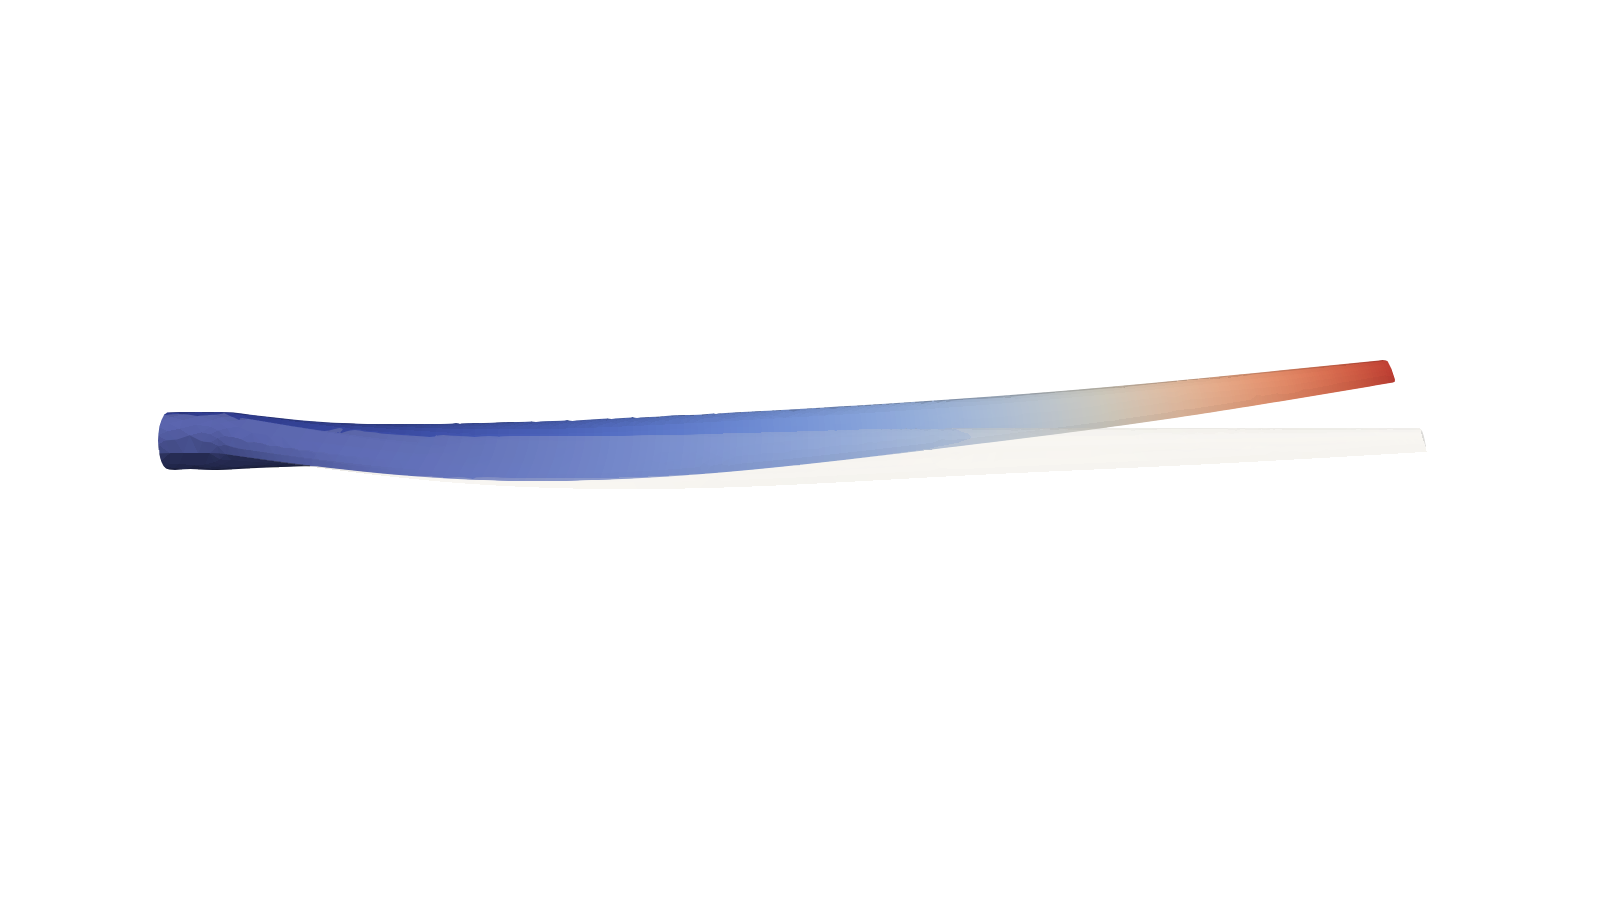
\includegraphics[width=\textwidth]{Figures/WindTurbineBladePODMode4.png}
        \caption{Mode 4}
    \end{subfigure}
    \hfill
    \begin{subfigure}[b]{0.3\textwidth}
        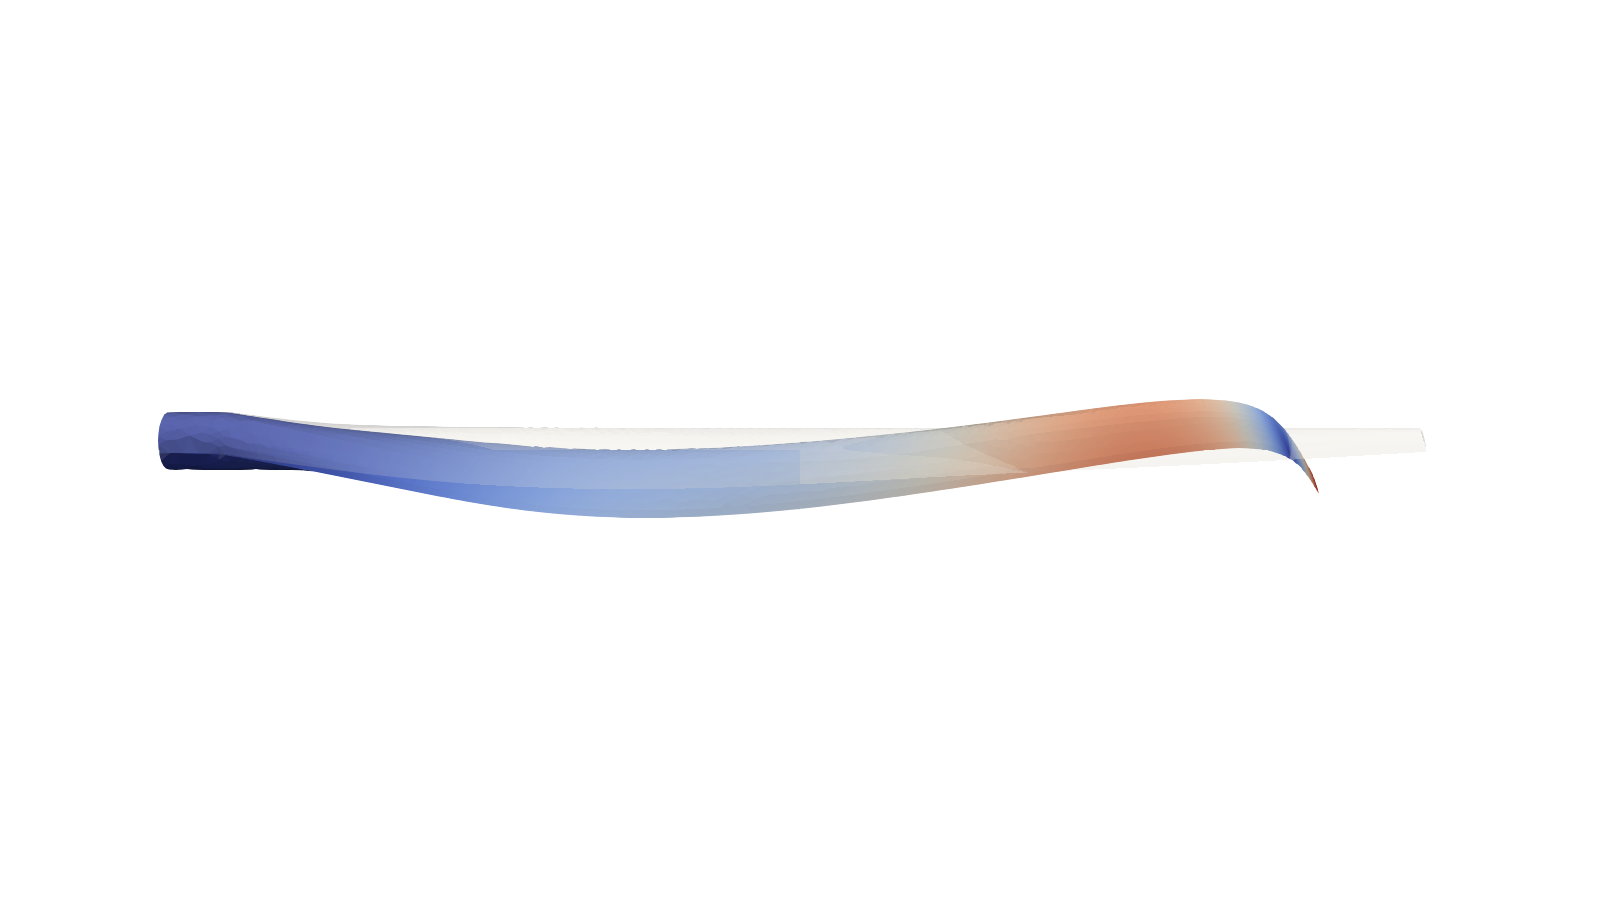
\includegraphics[width=\textwidth]{Figures/WindTurbineBladePODMode5.png}
        \caption{Mode 5}
    \end{subfigure}
    \hfill
    \begin{subfigure}[b]{0.3\textwidth}
        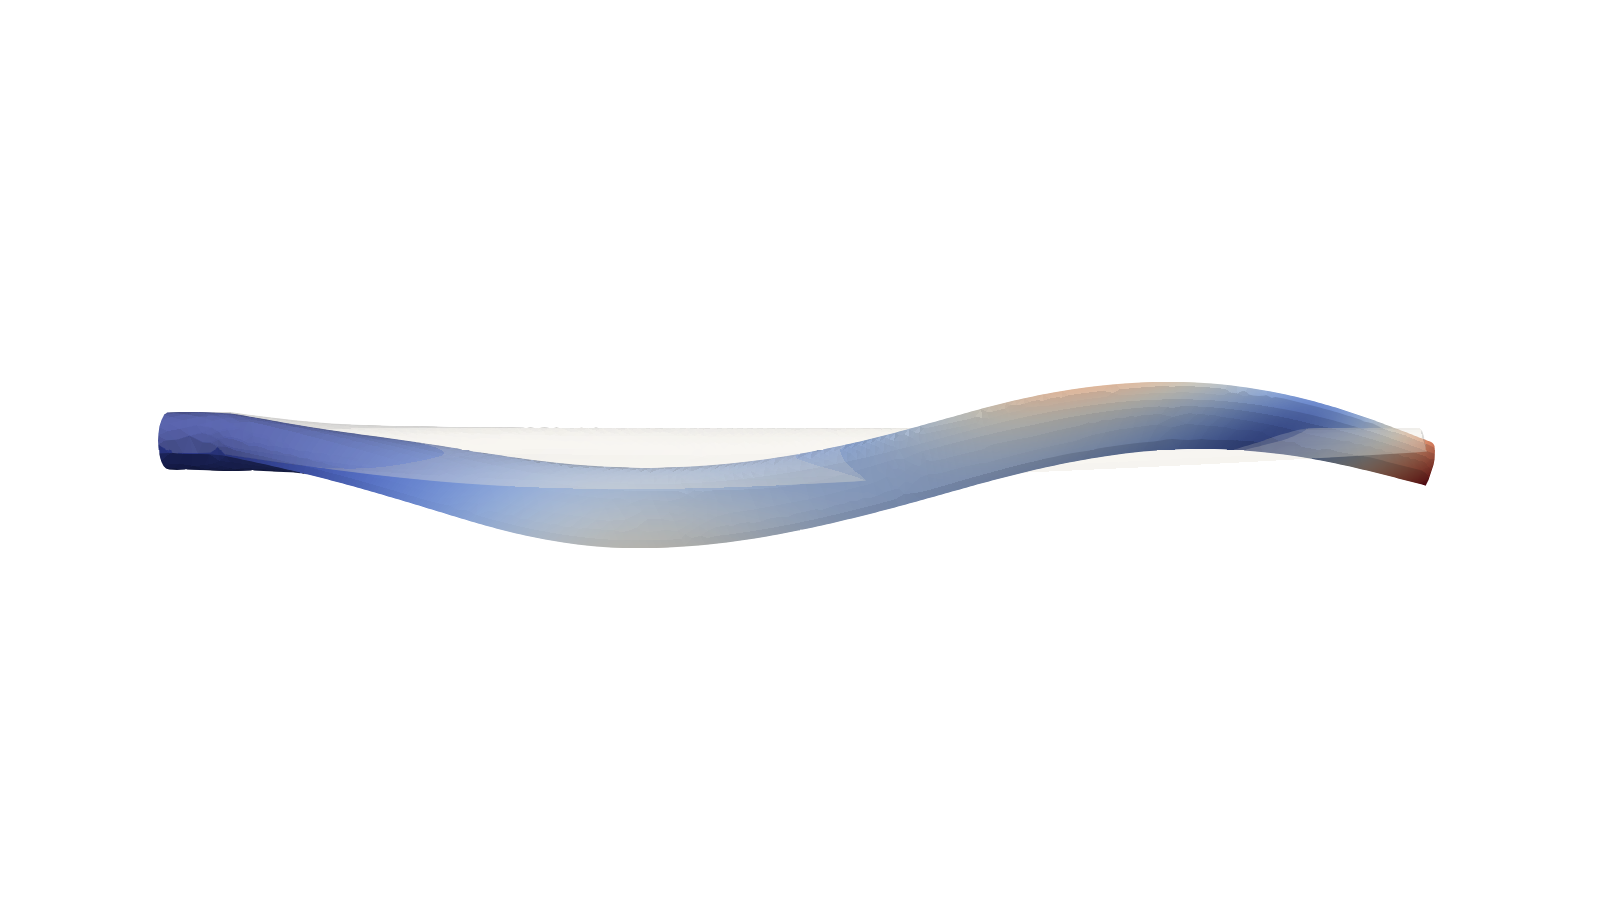
\includegraphics[width=\textwidth]{Figures/WindTurbineBladePODMode6.png}
        \caption{Mode 6}
    \end{subfigure}

    \caption{
    First six POD modes extracted from the full-order dynamic response of the wind turbine blade. These data-driven modes reflect dominant spatial deformation patterns learned from the high-fidelity simulation and serve as an efficient reduced basis for model order reduction.
    }
    \label{fig:blade_pod_modes}
\end{figure}


\paragraph{Results.}
A POD-based PROM is constructed using \(n=7\) modes based on maintaining a squared energy loss below \(\epsilon^2(n) \le 10^{-10}\). This criterion corresponds to a snapshot reconstruction error of \(\epsilon(n) = 10^{-5}\). 
When evaluated against the unseen test case loading, this 7-mode PROM achieves good predictive accuracy, exhibiting a relative error of approximately 0.14\% compared to the FOM. 
This relative error, denoted \(\mathbb{RE}_{2,\mathbf{u}}\), quantifies the difference between the PROM (\(\mathbf{\tilde{u}}\)) and FOM (\(\mathbf{u}\)) solutions over the trajectory for the test parameter case \(\boldsymbol{\mu}_{\text{test}}\), calculated using the time-accumulated 2-norm as:
\begin{equation} \label{eq:relative_error_def}
\mathbb{RE}_{2,\mathbf{u}} = 100\times\frac{\sqrt{\sum_{m=0}^{N_t} \|\mathbf{u}(t_m, \boldsymbol{\mu}_{\text{test}}) - \mathbf{\tilde{u}}(t_m, \boldsymbol{\mu}_{\text{test}})\|_2}}{\sqrt{\sum_{m=0}^{N_t} \|\mathbf{u}(t_m, \boldsymbol{\mu}_{\text{test}})\|_2}}.
\end{equation}
Qualitative comparisons of the tip displacement time histories and spatial deformation patterns are presented in Figure~\ref{fig:fom_vs_rom_tip} and Figure~\ref{fig:fom_rom_snapshots}, respectively.

Key quantitative performance metrics are summarised in Table~\ref{tab:rom_hrom_performance}. 
In terms of computational cost, the total wall-clock time was reduced from $348.41\,\text{s}$ for the FOM to $190.48\,\text{s}$ for the ROM, yielding an overall speed-up factor of $1.83\times$. 
This speed-up, while beneficial, is modest compared to the potential suggested by the drastic reduction in degrees of freedom ($N/n \approx 2526\times$). 
The discrepancy arises because, while the time required to solve the linear System of Equations (SoE) arising at each time step (or nonlinear iteration) is reduced dramatically (from \(0.20\,\text{s}\) for the FOM to \(8.3 \times 10^{-6}\,\text{s}\) for the ROM, yielding a speed-up factor of \(24\,096\times\)), the cost of assembling the reduced residual and Jacobian vectors dominates the computation. 
In the standard Galerkin projection framework used here, this assembly requires evaluating nonlinear terms over the full mesh ($13\,488$ elements), making its cost dependent on the FOM size. 
Therefore, despite the significant reduction in degrees of freedom, the computational complexity remains tied to the original FOM size. Addressing this assembly bottleneck is crucial for achieving substantial wall-clock time reductions and motivates the use of hyper-reduction techniques, which are introduced in the following section.

\subsection{Achieving real-time performance via hyper-reduction}
\label{sec:hrom_summary}

Despite the reduction in degrees of freedom achieved by the POD--Galerkin model (\(n = 7 \ll N = 17\,683\)), the total computational cost remains significantly influenced by the full-order discretization. This is because the residual and Jacobian assembly in the finite-element setting requires looping over all \(N_e = 13{,}488\) elements, with each elemental contribution accumulated into the global system.

Hyper-reduction techniques address this bottleneck by approximating the residual projection using only a subset of elements.  
Consider the full-order residual, assembled element-by-element,
\begin{equation}
\mathbf{R}(\boldsymbol{\Phi}\,\mathbf{q}) 
= \sum_{e=1}^{N_e} 
    \mathbf{L}_{e}^{\!T}\,
    \mathbf{R}_{e}\!\bigl(\mathbf{L}_{e}^{+}\,\boldsymbol{\Phi}\,\mathbf{q}\bigr),
\end{equation}
where \( \mathbf{R}_{e} \) is the local residual of mesh entity \(e\),  
\( \mathbf{L}_{e} \in \{0,1\}^{n_e \times N} \) is the Boolean scatter matrix that maps the \(n_e\) degrees of freedom (DOFs) associated with entity \(e\) into the global vector of size \(N\),  
and \( \mathbf{L}_{e}^{+} \in \{0,1\}^{n_e^+ \times N} \) gathers all DOFs needed by the stencil of the residual \( \mathbf{R}_{e} \).\footnote{The dependence of \( \mathbf{q} \) and \( \mathbf{R} \) on time and parameters \( \boldsymbol{\mu} \) is dropped here for simplicity of exposition.}  
For a finite element discretization, \( \mathbf{L}_{e}^{+} = \mathbf{L}_{e} \),  
while for a cell-centered finite volume or finite difference scheme, \( \mathbf{L}_{e}^{+} \) typically includes neighboring entities.  
Consequently, the reduced residual obtained by projection onto the POD basis \( \boldsymbol{\Phi} \) reads
\begin{equation}
\boldsymbol{\Phi}^{\!T}\mathbf{R}(\boldsymbol{\Phi}\,\mathbf{q}) 
= \sum_{e=1}^{N_e} 
    \bigl(\boldsymbol{\Phi}^{\!T}\mathbf{L}_{e}^{\!T}\bigr)
    \mathbf{R}_{e}\!\bigl(\mathbf{L}_{e}^{+}\,\boldsymbol{\Phi}\,\mathbf{q}\bigr)=\sum_{e=1}^{N_e}\boldsymbol{\Phi}_{e}^{\!T}
    \mathbf{R}_{e}\!\bigl(\mathbf{L}_{e}^{+}\,\boldsymbol{\Phi}\,\mathbf{q}\bigr),
\end{equation}
with \( \boldsymbol{\Phi}_{e} = \mathbf{L}_{e} \boldsymbol{\Phi} \in \mathbb{R}^{n_e \times n} \) the restriction of the reduced basis to the DOFs of element \(e\).

In this example, the hyper-reduction approximation is carried out using the Empirical Cubature Method (ECM). ECM selects a reduced mesh subset
\[
\widetilde{\mathcal{E}} \subset \{1,\dots,N_e\}, 
\quad |\widetilde{\mathcal{E}}| = n_e = 85,
\]
together with strictly positive cubature weights \( \{ \xi_{e} \}_{e \in \widetilde{\mathcal{E}}} \), such that the projected residual can be efficiently approximated as
\begin{equation}
\boldsymbol{\Phi}^{\!T}\mathbf{R}(\boldsymbol{\Phi}\,\mathbf{q})
\;\approx\;
\sum_{e \in \widetilde{\mathcal{E}}} \xi_{e} \,
\boldsymbol{\Phi}_{e}^{\!T} \, \mathbf{R}_{e}(\mathbf{L}_{e}^{+} \boldsymbol{\Phi}\,\mathbf{q}),
\end{equation}
where \( \boldsymbol{\Phi}_{e}^{\!T} := \boldsymbol{\Phi}^{\!T} \mathbf{L}_{e}^{\!T} \) denotes the restriction of the test space to the degrees of freedom associated with element \(e\).  
This formulation decouples the online cost from the full-order mesh while preserving projection accuracy.  
Other project-then-approximate hyper-reduction strategies, such as the Energy-Conserving Sampling and Weighting (ECSW)~\cite{Farhat2015} method, could also be employed.


A detailed derivation of the ECM formulation and the associated optimisation problem is provided in Chapters~\ref{chap:article1} and~\ref{chap:article2} and refs.~\cite{hernandez2017dimensional,hernandez2020multiscale}.  The remainder of this section summarises the computational impact of the resulting hyper‑reduced order model (HPROM).


Table~\ref{tab:rom_hrom_performance} consolidates the performance comparison of the FOM, the PROM, and the HPROM. Remarkably, the HPROM achieves a wall-clock time of only 5.91\,s, more than 32 times faster than the PROM and nearly 60 times faster than the FOM. This acceleration allows real-time execution of high-fidelity simulations, demonstrating the practical viability of PROM deployment in time-critical digital twin environments.

Figures~\ref{fig:fom_vs_rom_tip} and \ref{fig:fom_rom_snapshots} provide qualitative comparisons between the FOM, PROM, and HPROM solutions, highlighting the accuracy and effectiveness of the hyper-reduction approach in capturing the system's dynamic behavior.



\begin{table}[ht!]
\centering
\resizebox{\textwidth}{!}{% 
\begin{tabular}{@{}lccccccc@{}} 
\toprule 
\textbf{Computational Model} & 
\begin{tabular}[c]{@{}c@{}}$n$ \\ (\(N\) for FOM)\end{tabular} & 
\begin{tabular}[c]{@{}c@{}}$n_e$ \\ (\(N_e\) for FOM/PROM)\end{tabular} & 
\begin{tabular}[c]{@{}c@{}}\(\mathbb{RE}_{2,\mathbf{u}}\) \\ (\%)\end{tabular} & 
\begin{tabular}[c]{@{}c@{}}Wall-clock time \\ (\(s\))\end{tabular} & 
\begin{tabular}[c]{@{}c@{}}Wall-clock time \\ Speed-up\end{tabular} & 
\begin{tabular}[c]{@{}c@{}}Avg. SoE time \\ (\(s\))\end{tabular} & 
\begin{tabular}[c]{@{}c@{}}SoE time \\ speed-up\end{tabular} \\ 
\midrule 
FOM   & \(17\,683\) & \(13\,488\) & --   & 348.41 & --    & 0.20 & -- \\
PROM  & \(7\)       & \(13\,488\) & 0.14 & 190.48 & 1.83  & \(8.3 \times 10^{-6}\) & 24\,096 \\
HPROM & \(7\)       & \(\mathbf{85}\)     & 0.14 & \textbf{5.91} & \textbf{58.95} & \(8.3 \times 10^{-6}\) & 24\,096 \\
\bottomrule
\end{tabular}}% End resizebox
\caption{Performance comparison of the FOM, PROM, and HPROM for the wind turbine blade test case.}
\label{tab:rom_hrom_performance}
\end{table}


\begin{figure}[ht!]
    \centering
    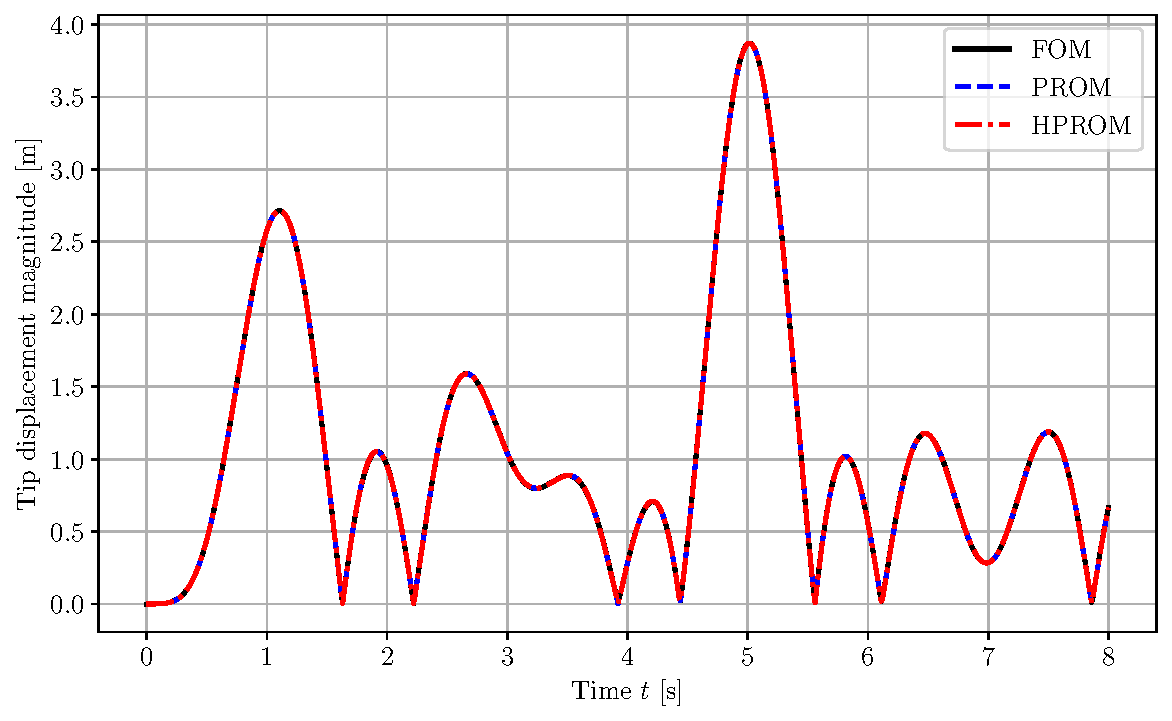
\includegraphics[width=0.75\textwidth]{Figures/tip_displacement_comparison.pdf}
    \caption{
    Time evolution of the wind turbine blade tip displacement under the test loading condition.
    }
    \label{fig:fom_vs_rom_tip}
\end{figure}

\begin{figure}[ht!]
    \centering

    % t = 1s
    \begin{subfigure}[b]{0.3\textwidth}
        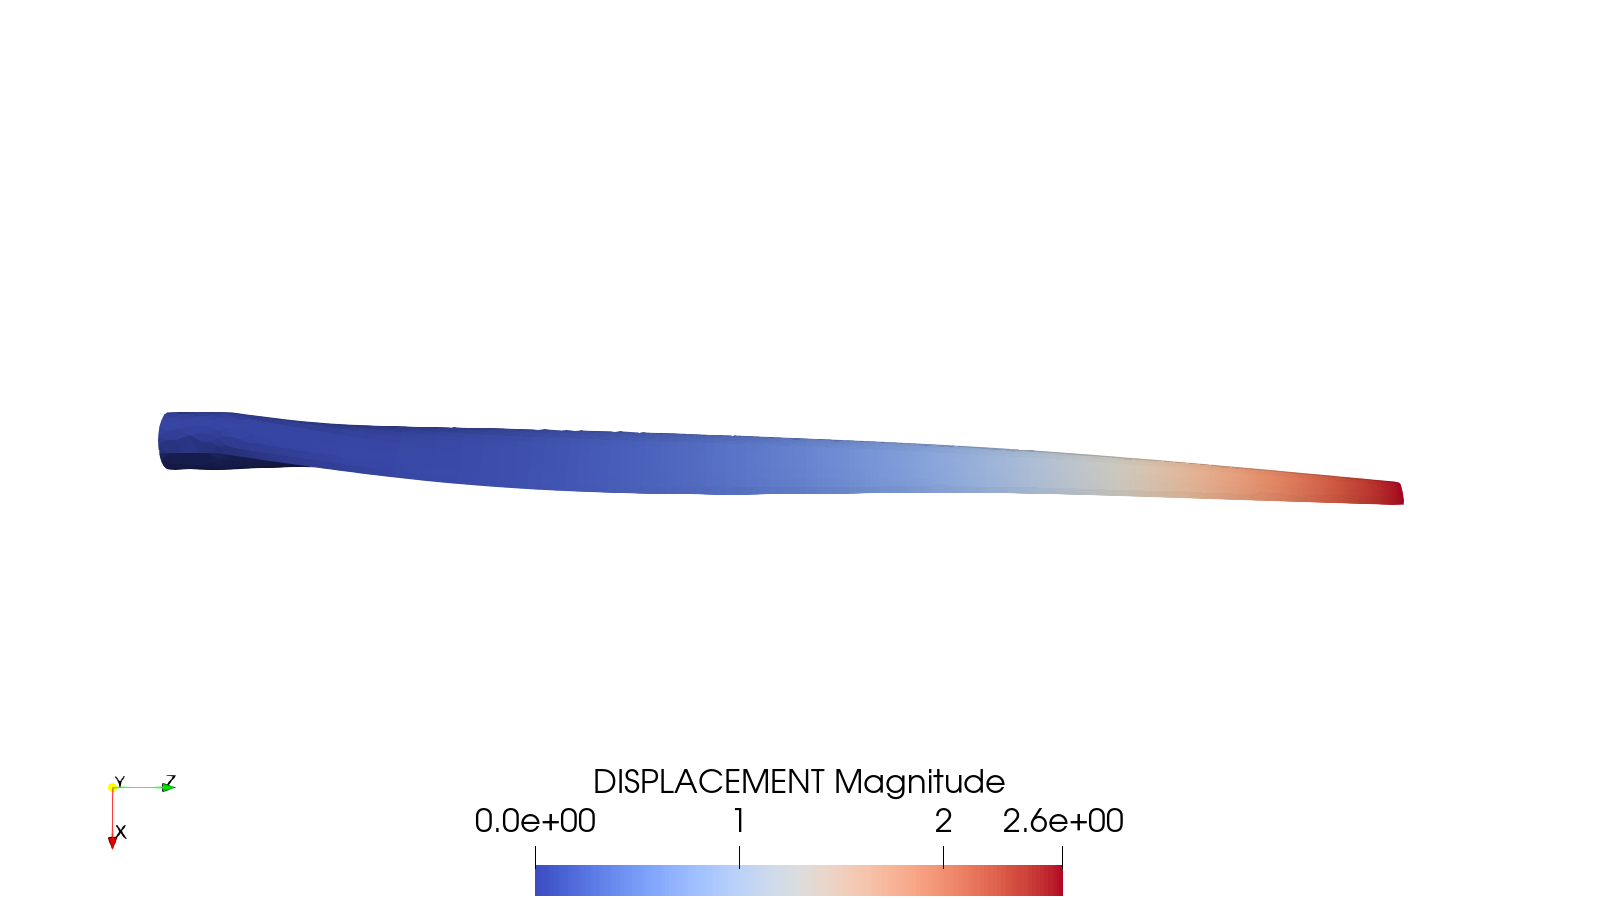
\includegraphics[width=\textwidth]{Figures/fom_t1.png}
        \caption{FOM at \(t = 1\,\text{s}\)}
    \end{subfigure}
    \hfill
    \begin{subfigure}[b]{0.3\textwidth}
        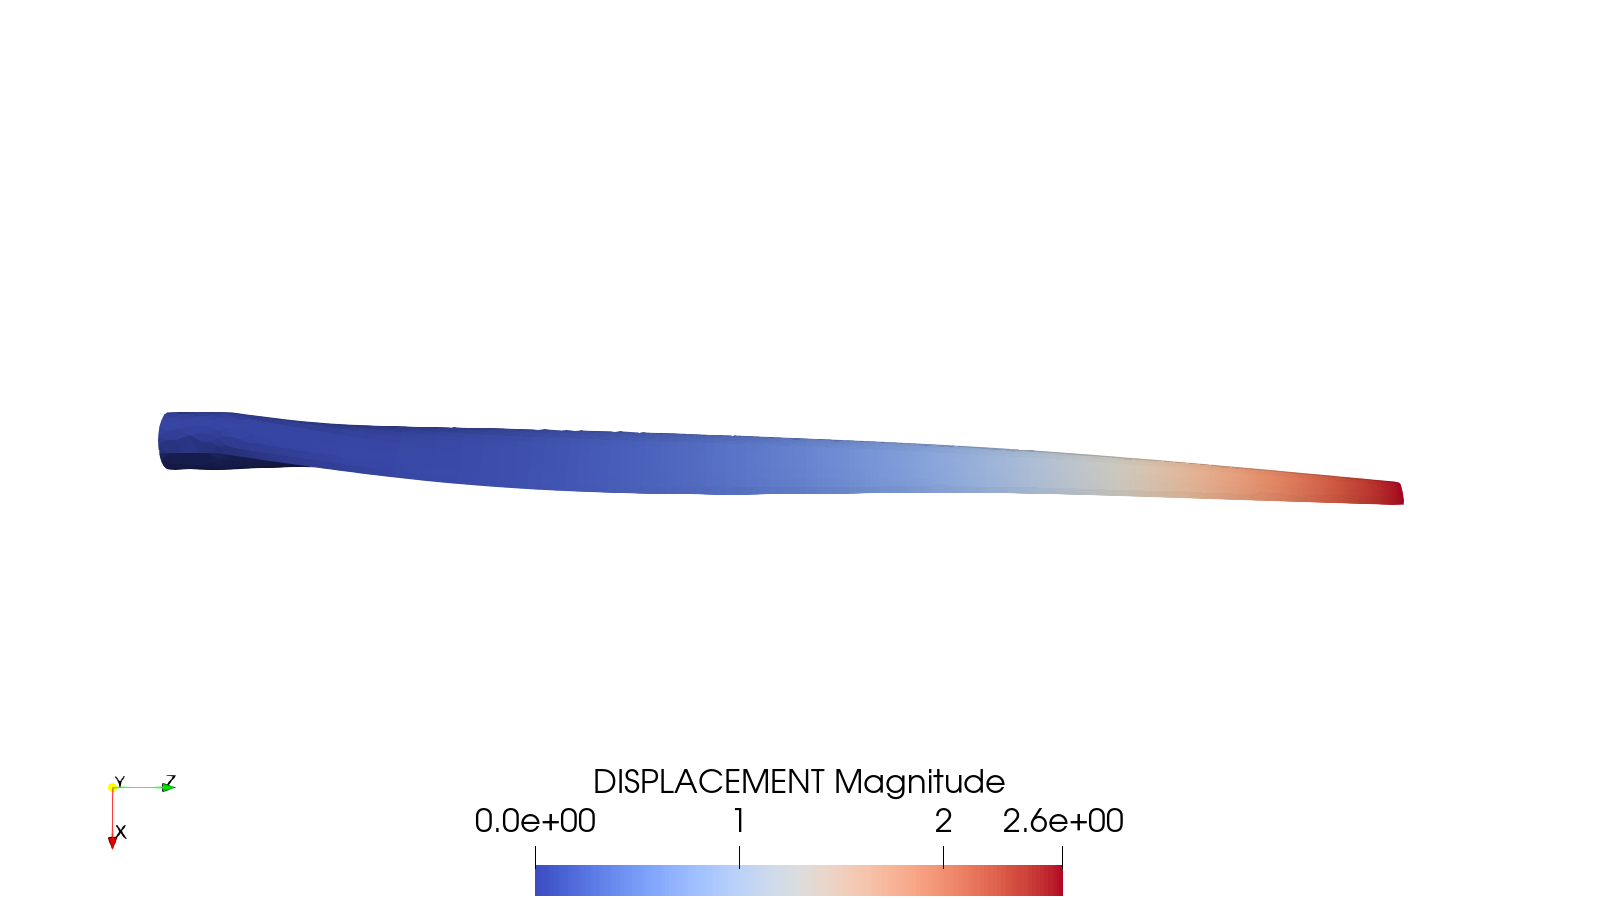
\includegraphics[width=\textwidth]{Figures/prom_t1.png}
        \caption{PROM at \(t = 1\,\text{s}\)}
    \end{subfigure}
    \hfill
    \begin{subfigure}[b]{0.3\textwidth}
        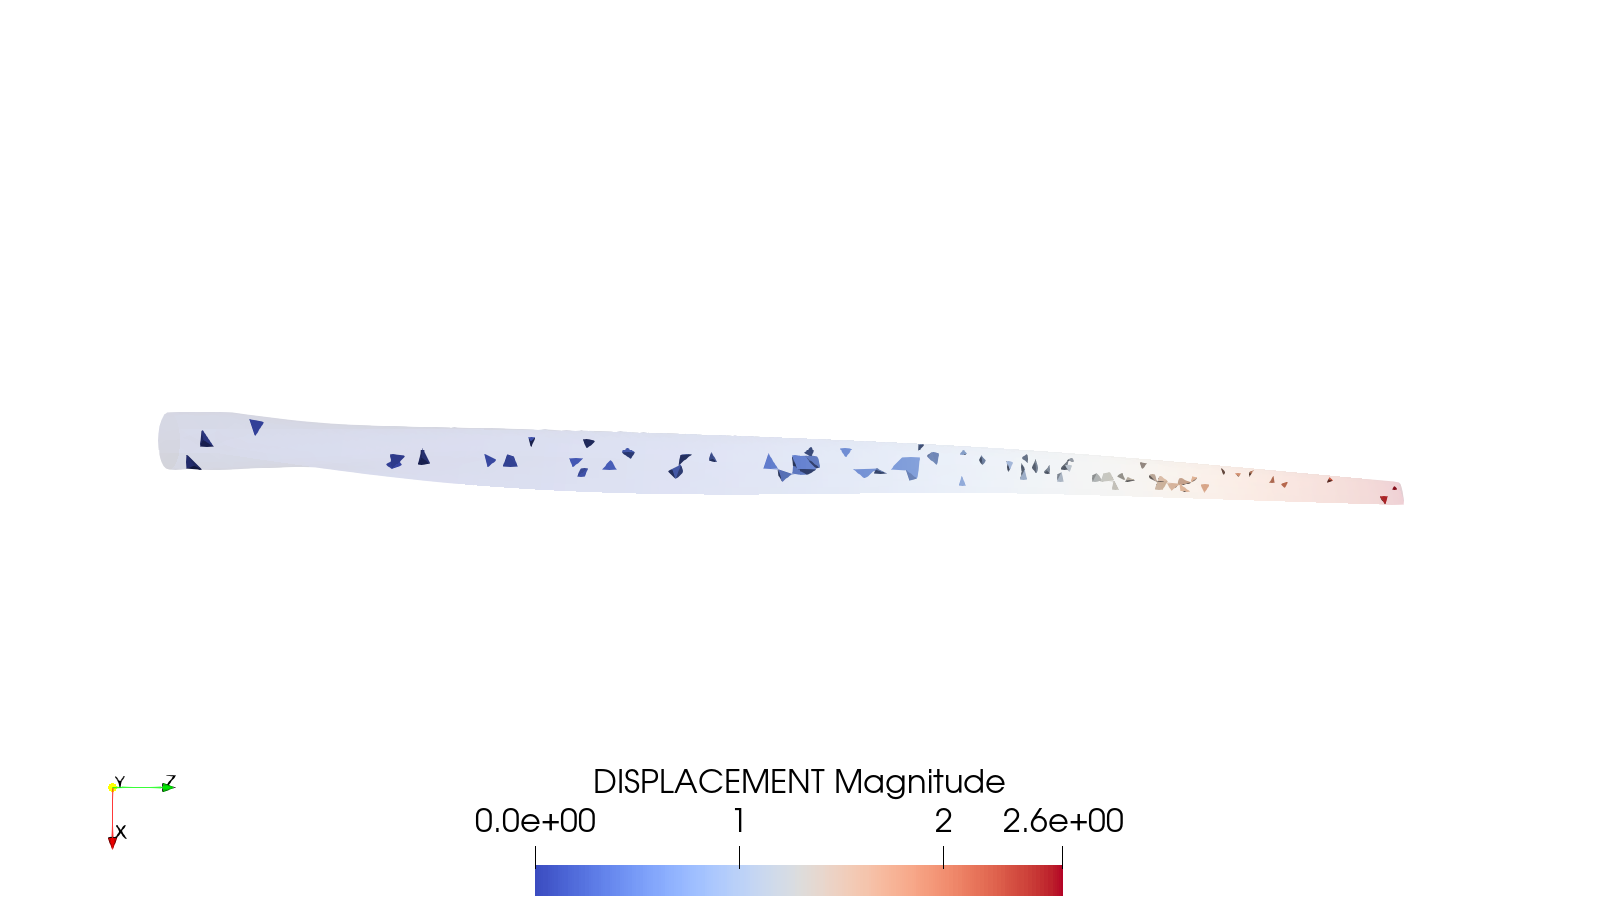
\includegraphics[width=\textwidth]{Figures/hprom_t1.png}
        \caption{HPROM at \(t = 1\,\text{s}\)}
    \end{subfigure}

    \vspace{1em}

    % t = 5s
    \begin{subfigure}[b]{0.3\textwidth}
        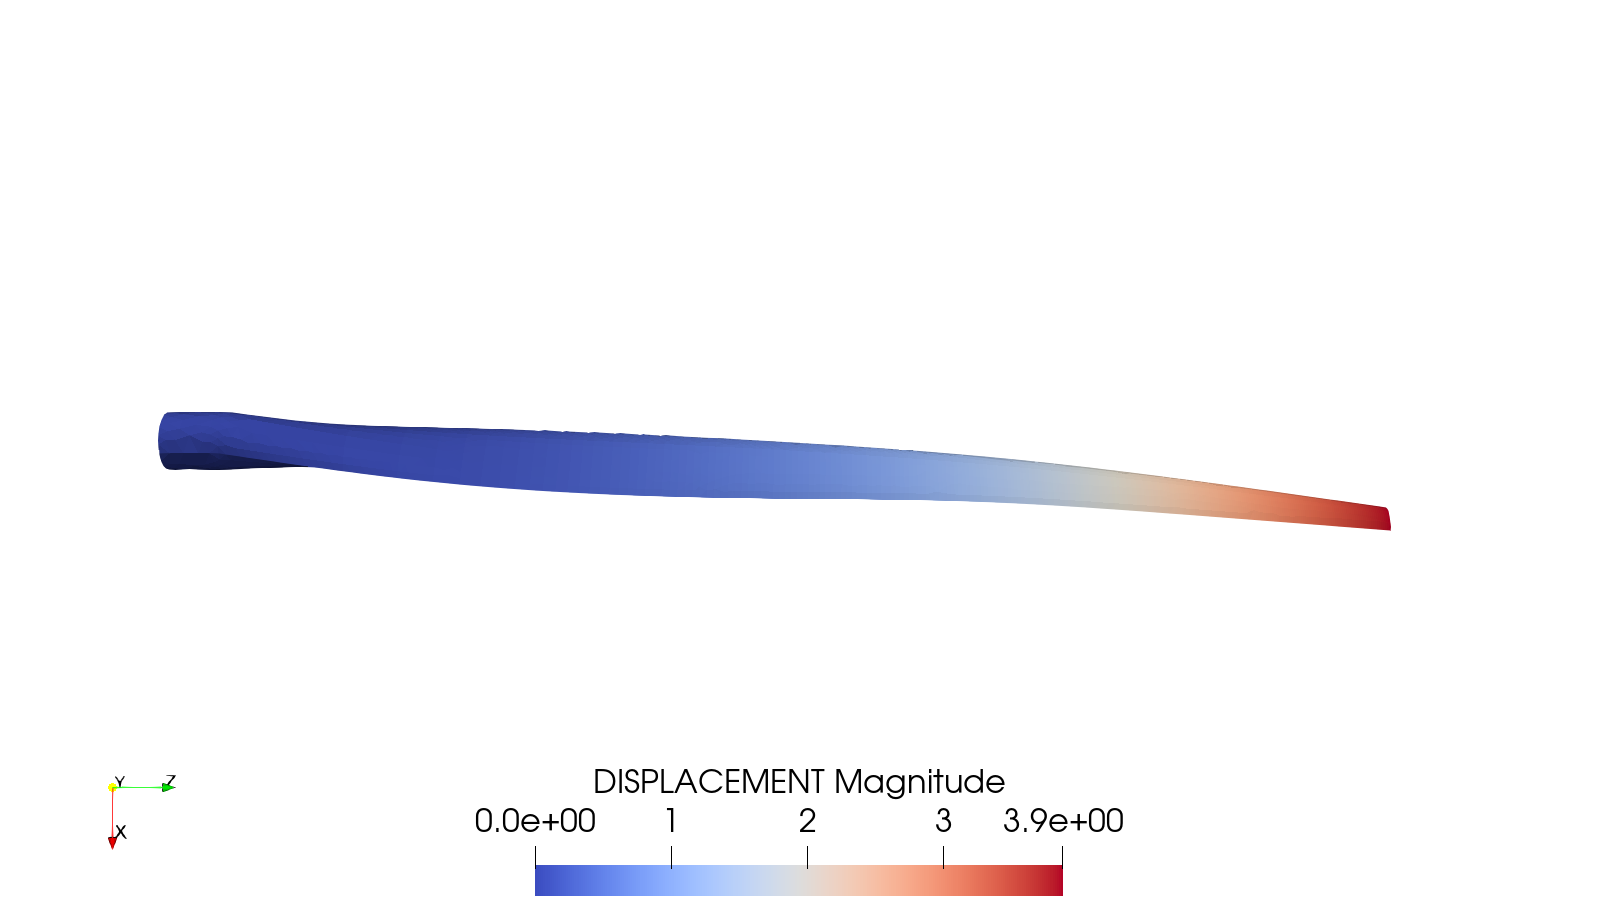
\includegraphics[width=\textwidth]{Figures/fom_t5.png}
        \caption{FOM at \(t = 5\,\text{s}\)}
    \end{subfigure}
    \hfill
    \begin{subfigure}[b]{0.3\textwidth}
        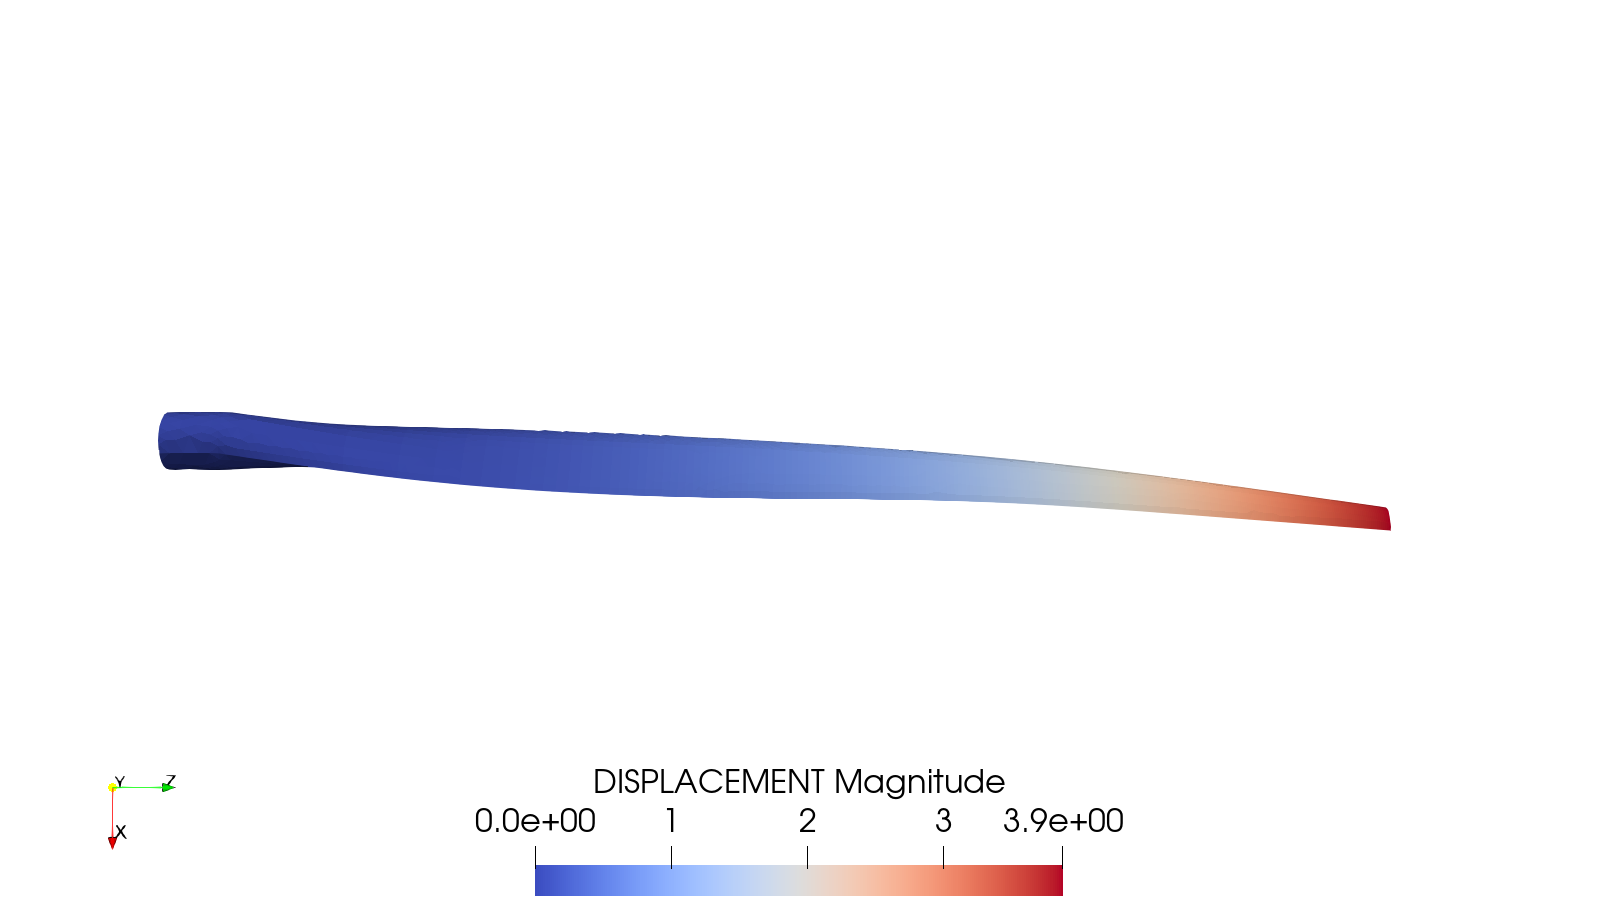
\includegraphics[width=\textwidth]{Figures/prom_t5.png}
        \caption{PROM at \(t = 5\,\text{s}\)}
    \end{subfigure}
    \hfill
    \begin{subfigure}[b]{0.3\textwidth}
        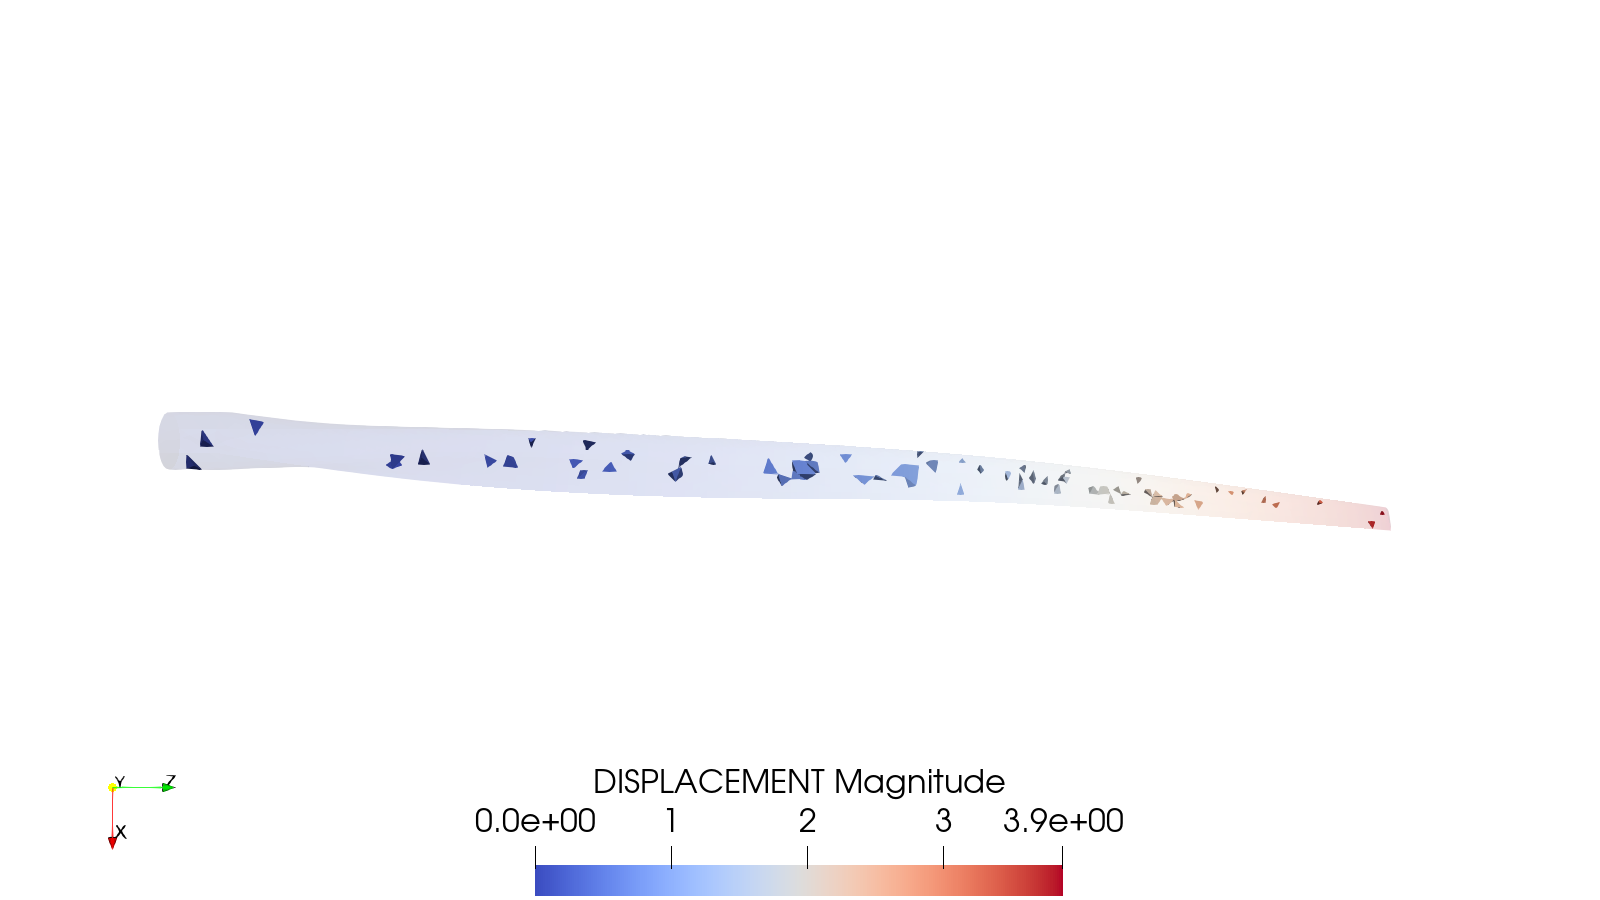
\includegraphics[width=\textwidth]{Figures/hprom_t5.png}
        \caption{HPROM at \(t = 5\,\text{s}\)}
    \end{subfigure}

    \caption{
    Spatial displacement fields of the wind turbine blade at two representative time instants during the test case simulation. Each row compares the FOM, PROM, and HPROM.
    }
    \label{fig:fom_rom_snapshots}
\end{figure}

\noindent
While the results confirm the effectiveness of POD-Galerkin for symmetric positive-definite problems, the next section shows that convection-dominated systems require a more robust projection, motivating the shift toward the LSPG framework.

\paragraph{Remark on industrial scalability.}
While the wind turbine blade example is solved efficiently using projection-based model reduction and hyper-reduction, it remains a relatively modest case in terms of size and parametric complexity. Nevertheless, it is derived from an actual industrial geometry and loading profile, and thus serves as a meaningful benchmark. In realistic engineering scenarios, featuring finer meshes, longer simulation horizons, richer material models, and high-dimensional parameter spaces, the offline construction of reduced-order models (e.g., snapshot generation, POD, and hyper-reduction via ECM) becomes a significant computational burden. These considerations motivate the need for parallel, HPC-enabled workflows to support scalable PROM construction for real-time digital twin applications. This broader perspective is discussed and addressed in the paper presented in Chapter~\ref{chap:article2}.

\section{Linear POD PROM for the model problem}
\label{sec:pod_prom_burgers}

\subsection{Parametric model problem and PROM setup}
\label{subsec:burgers_parametric_setup}

To evaluate the performance of linear subspace PROMs in convection-dominated regimes, the inviscid one-dimensional Burgers’ equation with a parametric source term is employed. This hyperbolic model problem, introduced in Chapter~\ref{sec:model_problem}, exhibits nonlinear wave propagation, shock formation, and non-symmetric residual operators, hallmarks of first-order hyperbolic PDEs that challenge standard projection methods due to their sharp gradients, low regularity, and parameter sensitivity.

For clarity of exposition, the governing equation is reprinted below in its parametric form:
\begin{equation}
\frac{\partial u}{\partial t} + u \frac{\partial u}{\partial x} = f(x; \mu_2),
\qquad
u(0, t) = \mu_1,
\label{eq:burgers_parametric}
\end{equation}
where \( \mu_1 \) denotes the left Dirichlet boundary condition, and \( \mu_2 \) modulates the spatial amplitude of the source term \( f(x; \mu_2) \). The full derivation of this model, including the weak form, finite element discretization with SUPG stabilization, time integration, and residual formulation, is presented in Section~\ref{sec:fem_discretization}.

The spatial domain \([0, 100]\) is discretized using 511 linear finite elements, yielding 512 nodes and therefore \( N = 512 \) spatial degrees of freedom. This discretization matches the setup introduced in Chapter~\ref{sec:model_problem} and is retained consistently throughout the PROM development.

The parametric domain is defined as
\[
\mathcal{D} = [4.25, 5.50] \times [0.015, 0.030],
\]
and is discretized using a uniform \( 3 \times 3 \) Cartesian grid (see Figure~\ref{fig:burgers_param_grid}), resulting in nine parameter configurations. For each \(\boldsymbol{\mu} \in \mathcal{D}\), a high-fidelity simulation is performed using backward Euler time integration and Newton–Raphson solvers, as described in Section~\ref{sec:fem_discretization}. Each trajectory consists of 500 time steps plus the initial condition, yielding 501 snapshots per parameter combination and resulting in the snapshot matrix \( \mathbf{S} \in \mathbb{R}^{N \times 4509} \).

\begin{figure}[ht!]
    \centering
    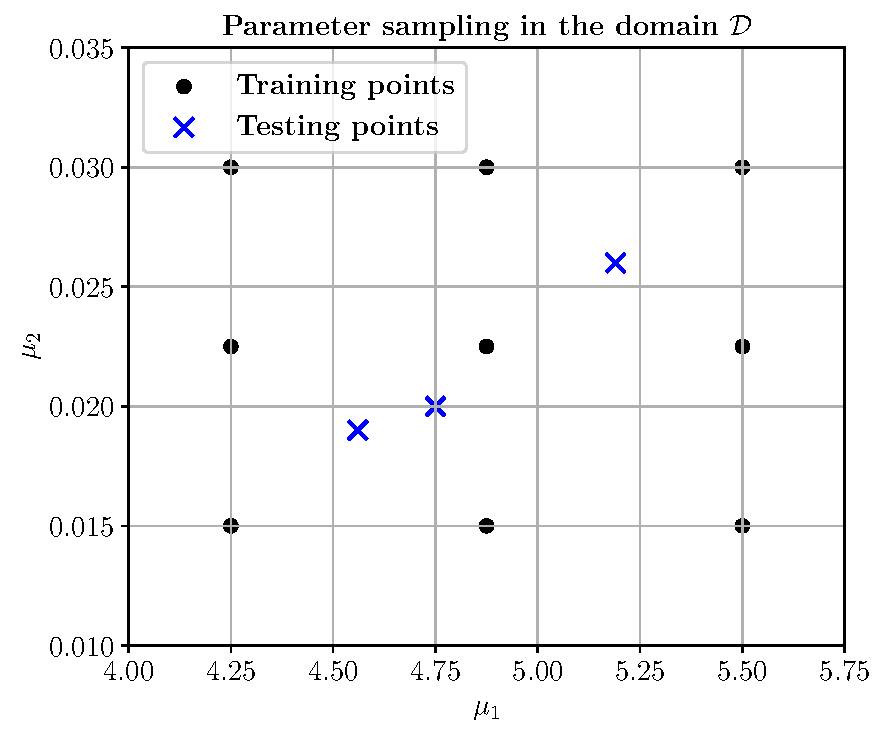
\includegraphics[width=0.65\textwidth]{Figures/parametric_domain.pdf}
    \caption{
        Training parameter combinations (black dots) and test configurations (blue crosses) in the parametric domain \( \mathcal{D} \subset \mathbb{R}^2 \).
    }
    \label{fig:burgers_param_grid}
\end{figure}

The nine training points \( \{\boldsymbol{\mu}^{(i)}_{\text{train}}\}_{i=1}^{9} \) form the basis of the offline stage for projection-based model reduction. In addition, three out-of-sample test configurations are selected within the domain to assess the generalization performance of the resulting PROM.

\subsection{Spectral decay and POD basis structure}
\label{subsec:pod_basis_structure}

The snapshot matrix \( \mathbf{S} \in \mathbb{R}^{N \times 4509} \), constructed from nine high-fidelity simulations across the parametric domain, is decomposed via SVD. The resulting singular values \( \{ \sigma_i \} \) quantify the projection error associated with truncating the left singular vectors, which define the reduced basis.

Figure~\ref{fig:singular_value_decay} presents the cumulative relative loss in linear energy as a function of the retained singular value index. The decay is notably slow, confirming that a high number of modes is required to achieve low approximation errors. This flat spectrum is a consequence of nonlinear transport phenomena, sharp wavefronts, and parametric variability, which reduce the compressibility of the solution manifold. This behavior is consistent with a system characterized by a high \emph{Kolmogorov \( n \)-width}~\cite{pinkus2012n}.

The vertical lines in Figure~\ref{fig:singular_value_decay} indicate the number of modes \( n \) needed to achieve different tolerance thresholds. Table~\ref{tab:mode_counts} summarizes the exact mode counts for the tolerances 
\[ \epsilon^2 = \{10^{-2}, 10^{-3}, 10^{-4}, 10^{-5}, 10^{-6}\}. \]

\begin{figure}[htbp]
    \centering
    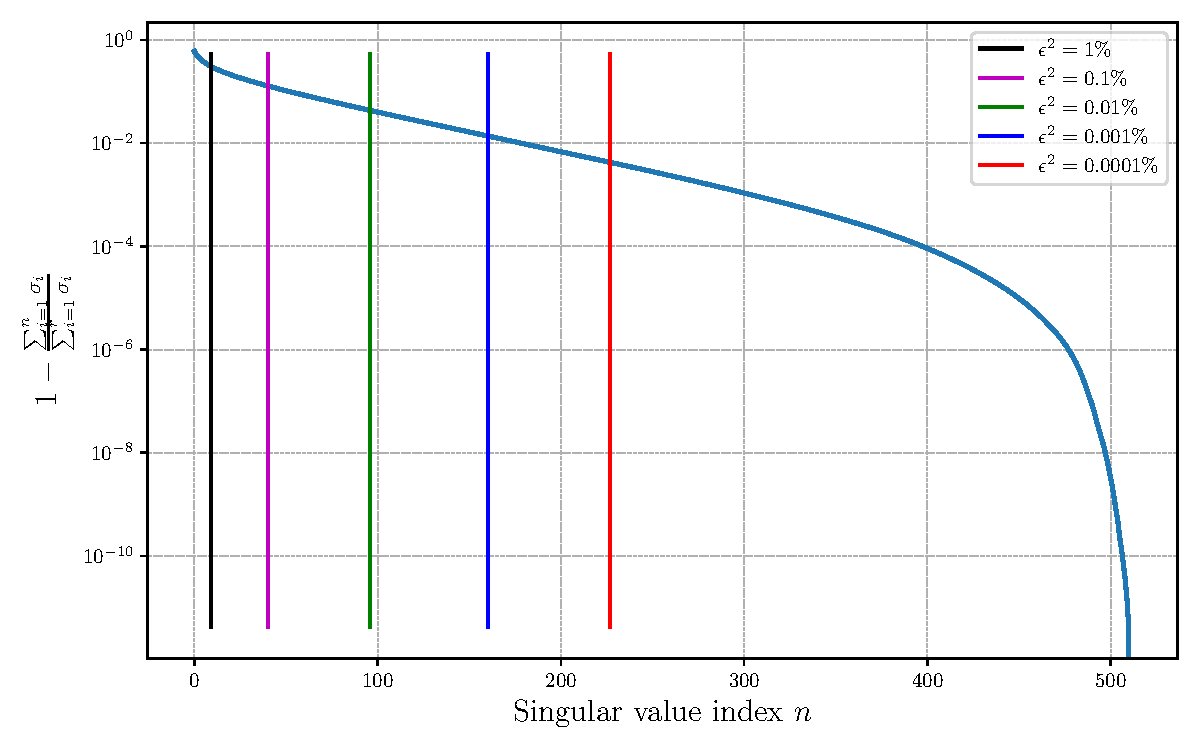
\includegraphics[width=0.7\textwidth]{Figures/singular_value_decay_linear_loss.pdf}
    \caption{Cumulative relative energy loss \( 1 - \sum_{i=1}^n \sigma_i / \sum_{i=1}^r \sigma_i \) for increasing number of retained singular values \( n \). Threshold lines show mode counts for selected tolerances \( \epsilon^2 \).}
    \label{fig:singular_value_decay}
\end{figure}

\begin{table}[!htbp]
    \centering
    \begin{tabular}{c|ccccc}
        \toprule
        \( \epsilon^2 \) & \( 10^{-2} \) & \( 10^{-3} \) & \( 10^{-4} \) & \( 10^{-5} \) & \( 10^{-6} \) \\
        \midrule
        \( n \) & 9 & 40 & 96 & 160 & 227 \\
        \bottomrule
    \end{tabular}
    \caption{Number of retained modes \( n \) for different squared tolerance thresholds \( \epsilon^2 \).}
    \label{tab:mode_counts}
\end{table}

Figure~\ref{fig:first6_pod_modes} displays the first six left singular vectors (POD modes). The modes exhibit increasing spatial oscillations and steepening fronts, aligned with the structure of propagating nonlinear waves.

\begin{figure}[!htbp]
    \centering
    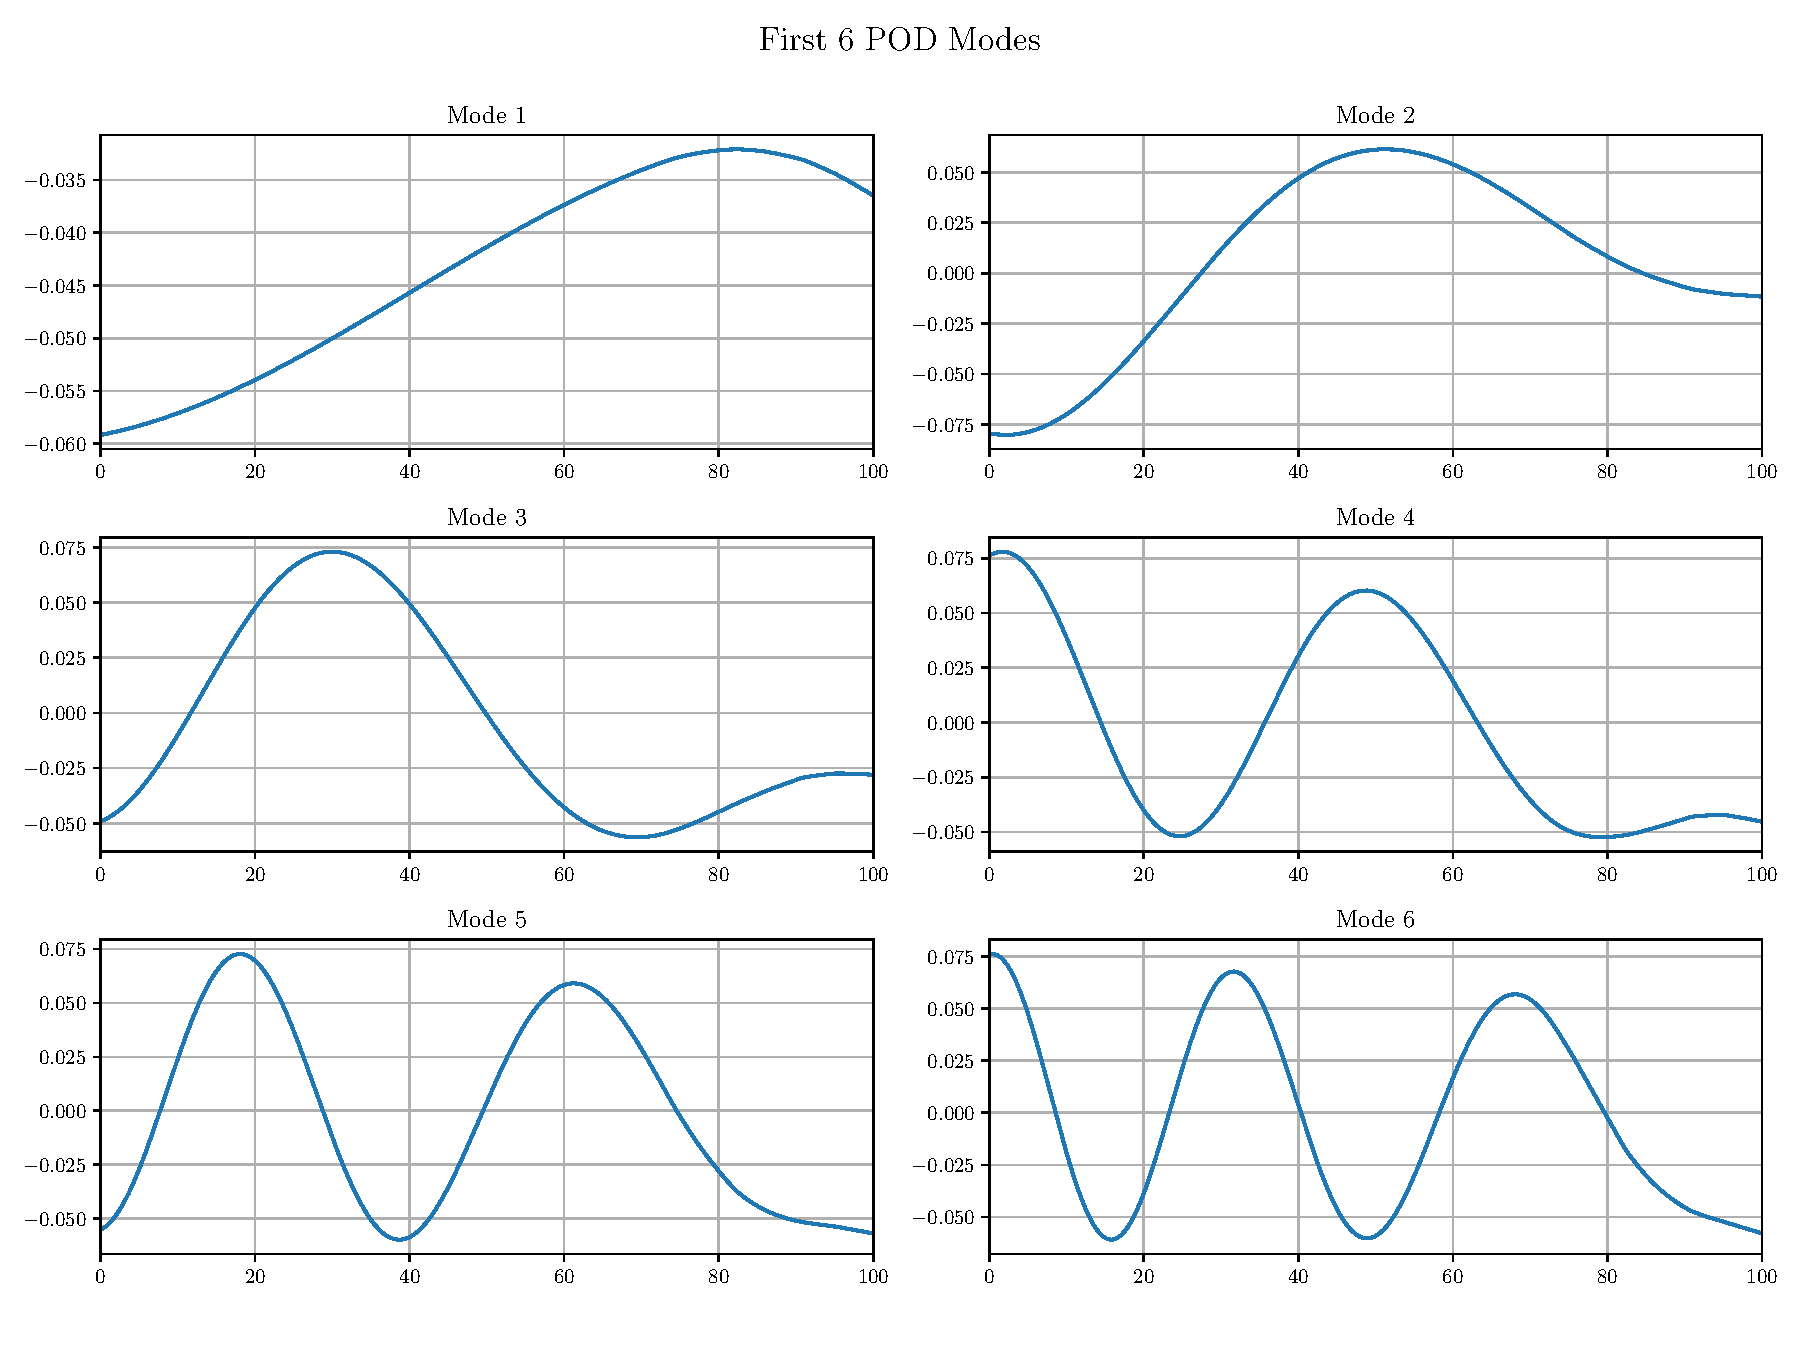
\includegraphics[width=0.75\textwidth]{Figures/first_6_modes.pdf}
    \caption{First six POD modes extracted from the SVD of the snapshot matrix. Each mode is defined over the domain \( x \in [0,100] \) with \( N = 512 \) spatial degrees of freedom.}
    \label{fig:first6_pod_modes}
\end{figure}

\subsection{Galerkin vs. LSPG projection for PROMs and the limitations of linear subspaces}
\label{subsec:galerkin_lspg_comparison}

Although the Galerkin projection offers optimality guarantees for symmetric positive-definite (SPD) operators, in convection-dominated flows, such as the one-dimensional inviscid Burgers equation considered here, the system operators are non-symmetric and dominated by transport terms, leading to suboptimal performance and potential instabilities with the Galerkin projection~\cite{carlberg2011efficient, carlberg2017galerkin}.

To address these limitations, the LSPG formulation replaces the orthogonality condition with a residual minimization principle, solving at each time step and parameter instance the nonlinear least-squares problem:
\begin{equation}
\min_{\mathbf{q}(t,\boldsymbol{\mu})} \; 
\tfrac{1}{2} \left\| 
\mathbf{R}\bigl(\boldsymbol{\Phi}\,\mathbf{q}(t,\boldsymbol{\mu});\,t,\boldsymbol{\mu}\bigr) 
\right\|_2^2.
\end{equation}
This optimization yields the first-order optimality condition
\begin{equation}\label{eq:lspg_residual}
\boldsymbol{\Phi}^{\!T}\,
\mathbf{J}^{\!T}\bigl(\boldsymbol{\Phi}\,\mathbf{q}(t,\boldsymbol{\mu});\,t,\boldsymbol{\mu}\bigr)\,
\mathbf{R}\bigl(\boldsymbol{\Phi}\,\mathbf{q}(t,\boldsymbol{\mu});\,t,\boldsymbol{\mu}\bigr)
= \mathbf{0},
\end{equation}
defining the LSPG reduced residual system
\begin{equation}
\mathbf{R}_{r}^{\text{LSPG}}\bigl(\mathbf{q}(t,\boldsymbol{\mu});\,t,\boldsymbol{\mu}\bigr) 
:= \boldsymbol{\Phi}^{\!T}\,
\mathbf{J}^{\!T}\bigl(\boldsymbol{\Phi}\,\mathbf{q}(t,\boldsymbol{\mu});\,t,\boldsymbol{\mu}\bigr)\,
\mathbf{R}\bigl(\boldsymbol{\Phi}\,\mathbf{q}(t,\boldsymbol{\mu});\,t,\boldsymbol{\mu}\bigr)
\;\in\; \mathbb{R}^n.
\end{equation}

This nonlinear reduced system is typically solved with Newton iterations, requiring the reduced LSPG Jacobian
\begin{equation}\label{eq:lspg_reduced_jacobian}
\mathbf{J}_{r}^{\text{LSPG}}\bigl(\mathbf{q}(t,\boldsymbol{\mu});\,t,\boldsymbol{\mu}\bigr) 
= \boldsymbol{\Phi}^{\!T}\,
\mathbf{J}^{\!T}\bigl(\boldsymbol{\Phi}\,\mathbf{q}(t,\boldsymbol{\mu});\,t,\boldsymbol{\mu}\bigr)\,
\mathbf{J}\bigl(\boldsymbol{\Phi}\,\mathbf{q}(t,\boldsymbol{\mu});\,t,\boldsymbol{\mu}\bigr)\,
\boldsymbol{\Phi}
\;\in\;\mathbb{R}^{n\times n}.
\end{equation}


The LSPG formulation enhances robustness for convection-dominated and non-SPD systems by relaxing the strict projection orthogonality and instead enforcing residual minimization in the full-order space (see Chapter~\ref{chap:article1} for a complete derivation).

To compare the performance of the Galerkin and LSPG projection methods, reduced-order solutions are evaluated for three test parameter configurations outside the training set: $\boldsymbol{\mu}_1 = [4.75,\, 0.0200]$, $\boldsymbol{\mu}_2 = [4.56,\, 0.0190]$, and $\boldsymbol{\mu}_3 = [5.19,\, 0.0260]$. Each model is tested across multiple truncation tolerances, and predictive accuracy is assessed through quantitative and qualitative comparisons with the corresponding FOM solutions.

\textbf{Quantitative assessment.}
To evaluate the predictive accuracy of the Galerkin and LSPG reduced-order models, the following relative error metric is adopted:
\begin{equation}
	\label{eq:error-metric}
	\mathbb{RE}_{2, \text{QoI}}(\boldsymbol{\mu}^\star) = 100\times \frac{\sqrt{\displaystyle \sum_{m=0}^{N_t} \left\|\,\text{QoI}_m(\boldsymbol{\mu^\star}) - \widetilde{\text{QoI}}_m (\boldsymbol{\mu^\star})\, \right \|_2^2}} {\sqrt{\sum\limits_{m=0}^{N_t} \left \|\,\text{QoI}_m (\boldsymbol{\mu^\star})\,\right\|_2^2}},
\end{equation}
where the quantity of interest (QoI) is the full solution vector $\mathbf{u}_m$, and the error is accumulated over the complete time horizon $[0, 25\,\text{s}]$.

Figure~\ref{fig:prom_multitols_finaltime} compares Galerkin and LSPG predictions against the FOM solution at final time $t = 25\,\text{s}$ for the test case $\boldsymbol{\mu}_2 = [4.56,\, 0.0190]$, across four different tolerances ($10^{-2}$ to $10^{-5}$). Both PROMs benefit from increasing basis resolution; however, LSPG consistently offers better agreement with the FOM for tolerances $\epsilon^2 \leq 10^{-3}$, while Galerkin suffers from visible post-shock oscillations.

\begin{figure}[htbp]
    \centering
    \begin{subfigure}{0.48\textwidth}
        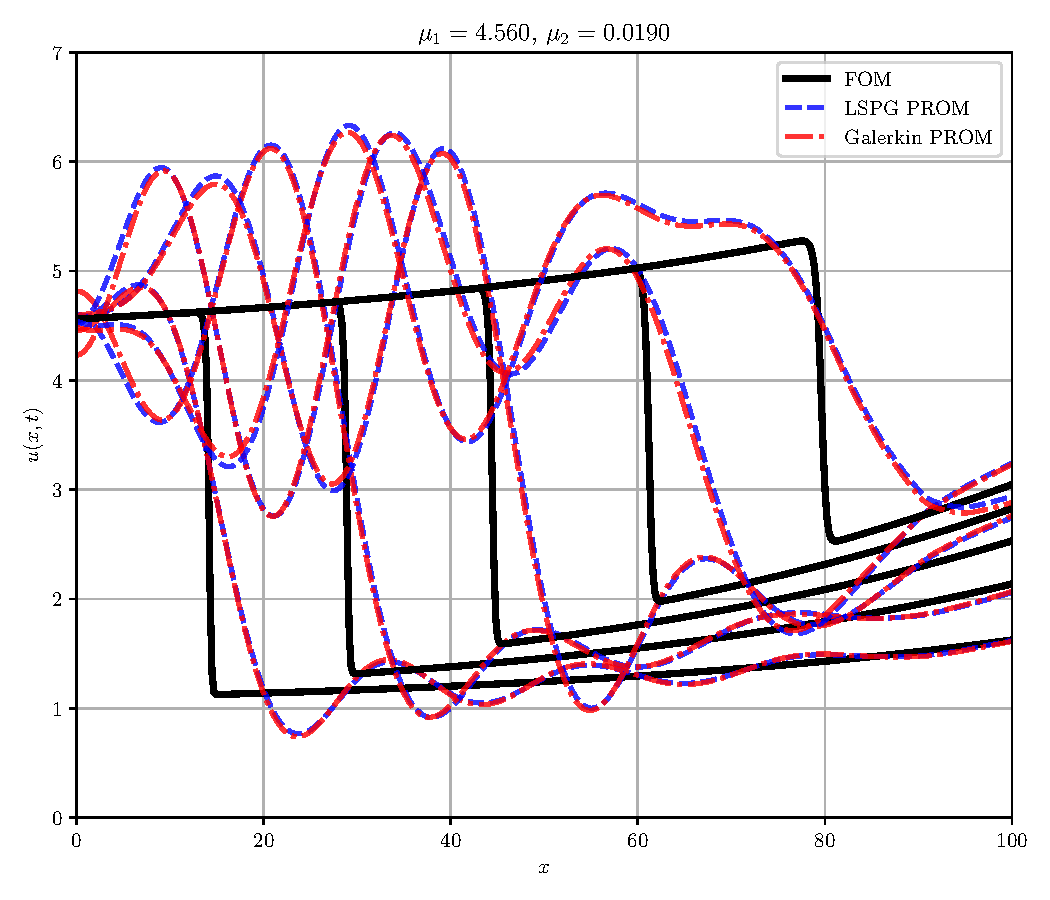
\includegraphics[width=\textwidth]{Figures/fom_pod_mu1_4.560_mu2_0.0190_tol_1e-02_modes_9.pdf}
        \caption{$\epsilon^2 = 10^{-2}$ ($n = 9$)}
    \end{subfigure}
    \hfill
    \begin{subfigure}{0.48\textwidth}
        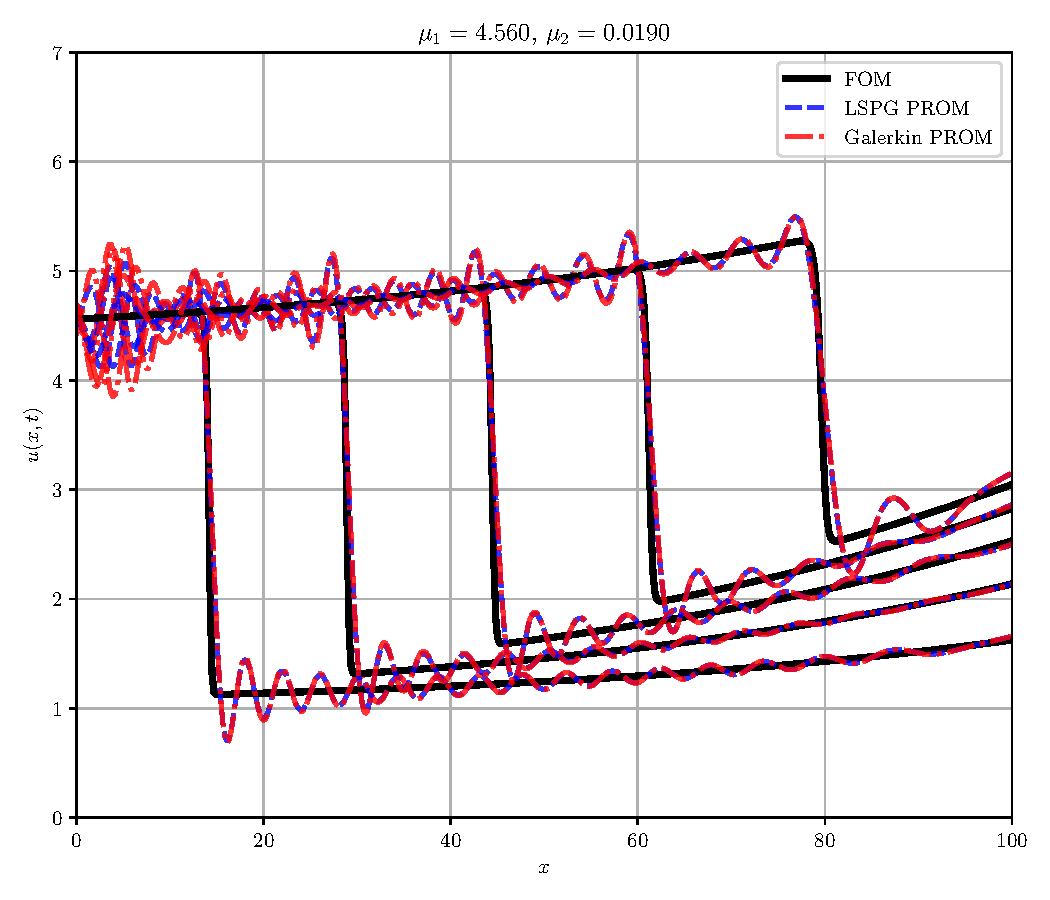
\includegraphics[width=\textwidth]{Figures/fom_pod_mu1_4.560_mu2_0.0190_tol_1e-03_modes_40.pdf}
        \caption{$\epsilon^2 = 10^{-3}$ ($n = 40$)}
    \end{subfigure}

    \vspace{0.5em}

    \begin{subfigure}{0.48\textwidth}
        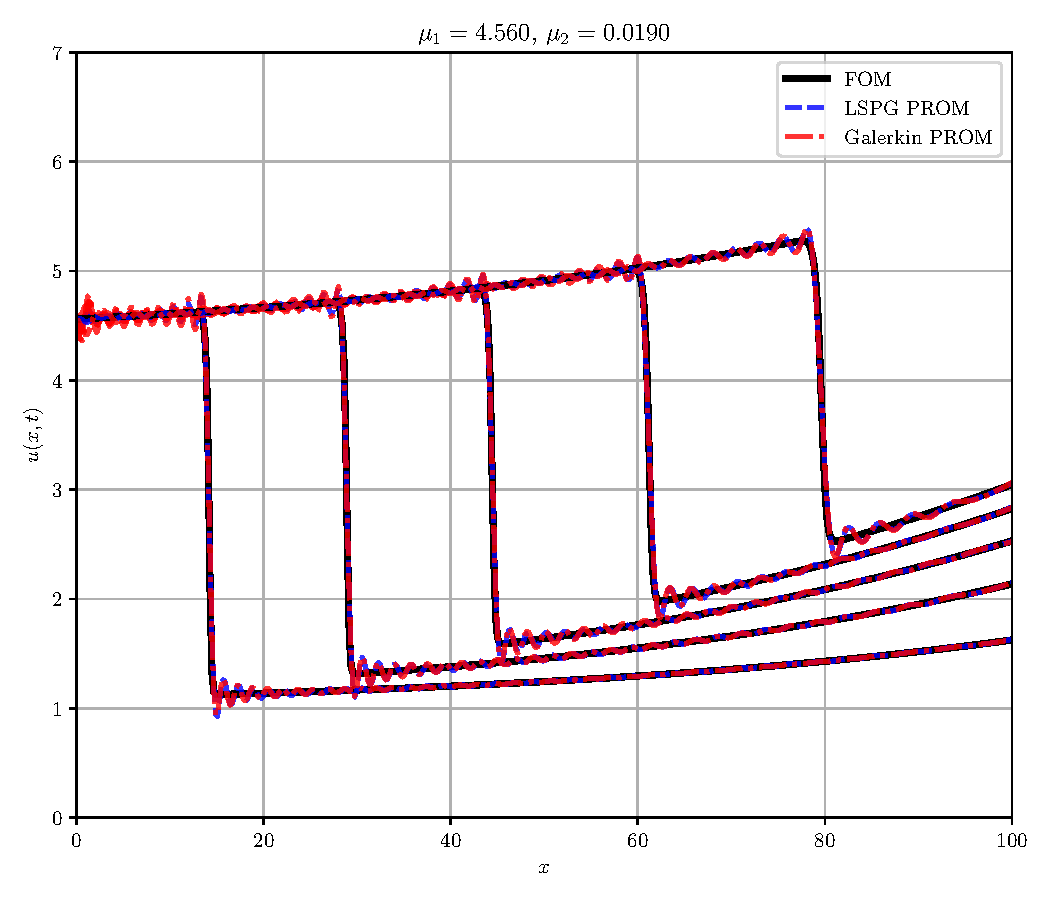
\includegraphics[width=\textwidth]{Figures/fom_pod_mu1_4.560_mu2_0.0190_tol_1e-04_modes_96.pdf}
        \caption{$\epsilon^2 = 10^{-4}$ ($n = 96$)}
    \end{subfigure}
    \hfill
    \begin{subfigure}{0.48\textwidth}
        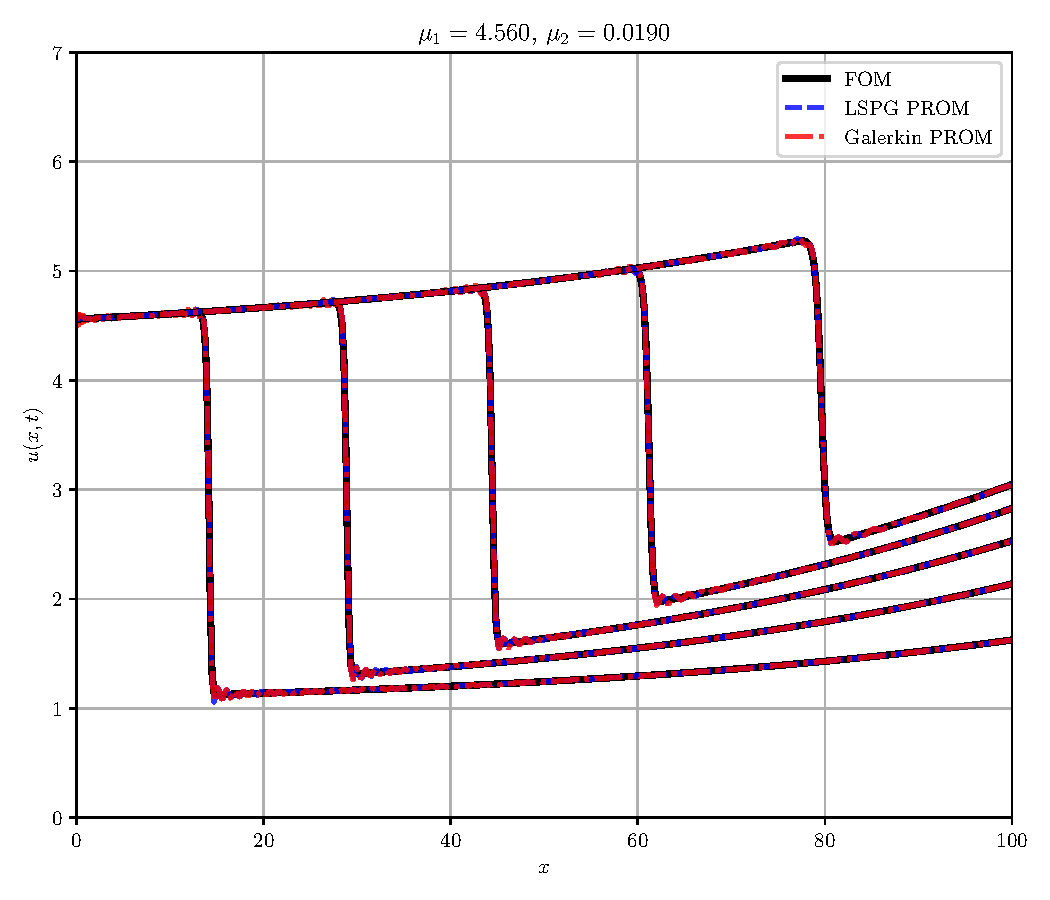
\includegraphics[width=\textwidth]{Figures/fom_pod_mu1_4.560_mu2_0.0190_tol_1e-05_modes_160.pdf}
        \caption{$\epsilon^2 = 10^{-5}$ ($n = 160$)}
    \end{subfigure}
    \caption{
        Galerkin and LSPG PROM predictions at $t = 25\,\text{s}$ for $\boldsymbol{\mu}^\star = [4.56,\, 0.0190]$ using different truncation tolerances. FOM reference is in black.
    }
    \label{fig:prom_multitols_finaltime}
\end{figure}

To summarize performance over all test cases, the maximum relative error is defined as:
\begin{equation*} 
	\mathbb{RE}_{2, \text{QoI}}^{\max} = \max_{\boldsymbol{\mu}_1, \boldsymbol{\mu}_2, \boldsymbol{\mu}_3} 
	\mathbb{RE}_{2, \text{QoI}} (\boldsymbol{\mu}),
\end{equation*}
and report it for each projection method and tolerance in Table~\ref{tab:prom_errors_summary}. The LSPG method outperforms Galerkin in all but the most severe truncation ($\epsilon^2 = 10^{-2}$), where the PROM dimension is insufficient to capture key features of the dynamics. Across all other settings, LSPG consistently yields lower maximum errors.

\begin{table}[!htbp]
    \centering
    \begin{tabular}{c c c c}
        \toprule
        \begin{tabular}[c]{@{}c@{}}Tolerance\\ $\epsilon^2$\end{tabular} & 
        \begin{tabular}[c]{@{}c@{}}Modes\\ $n$\end{tabular} & 
        \begin{tabular}[c]{@{}c@{}}Galerkin\\ $\mathbb{RE}_{2, \mathbf{u}}^{\max}$ (\%)\end{tabular} & 
        \begin{tabular}[c]{@{}c@{}}LSPG\\ $\mathbb{RE}_{2, \mathbf{u}}^{\max}$ (\%)\end{tabular} \\
        \midrule
        \( 10^{-2} \)  & 9    & 20.70 & 21.60 \\
        \( 10^{-3} \)  & 40   & 5.46  & 4.60  \\
        \( 10^{-4} \)  & 96   & 1.27  & 1.09  \\
        \( 10^{-5} \)  & 160  & 0.35  & 0.33  \\
        \( 10^{-6} \)  & 210  & 0.10  & 0.10  \\
        \bottomrule
    \end{tabular}
    \caption{Maximum relative error across three test configurations for Galerkin and LSPG PROMs at final time.}
    \label{tab:prom_errors_summary}
\end{table}

\textbf{Qualitative assessment.}
Figure~\ref{fig:prom_comparison_test1} shows the predicted solution at $t = 5\,\text{s}$ for the test configuration $\boldsymbol{\mu} = [4.75,\, 0.0200]$, using a reduced basis constructed with $\epsilon^2 = 10^{-4}$ (i.e., $n = 96$ modes). Both Galerkin and LSPG PROMs exhibit noticeable oscillations near the moving shock and in the post-shock region, reflecting the limitations of fixed linear subspaces in representing sharp, transport-dominated dynamics, an issue that arises independently of the projection method (i.e., standard POD reconstruction).
While neither approach yields highly accurate reconstructions, the LSPG projection consistently achieves slightly lower amplitude deviations compared to Galerkin.

These discrepancies are attributed to the residual-minimizing nature of LSPG, which improves robustness for hyperbolic, non-symmetric problems. Although the benefits of LSPG are moderate in this moderately reduced setting, the differences become more consequential in challenging configurations. In particular, while both PROMs remain stable in this benchmark case, the suboptimality of Galerkin can lead to unstable behavior or even numerical blow-up in more sensitive or industrial-scale applications, such as turbulent compressible flow simulations~\cite{carlberg2017galerkin}, underscoring the importance of careful projection design.

Altogether, these observations highlight the fundamental limitations imposed by the Kolmogorov $n$-width barrier when relying on linear trial subspaces. While increasing the number of modes can eventually improve accuracy (e.g., by reducing oscillations in the present case), overcoming the barrier often demands retaining an impractically large basis, which defeats the purpose of reduced-order modeling. \textbf{This motivates the transition to nonlinear manifold projection-based reduced-order models}, which relax the linear subspace constraint to better capture complex dynamics, a direction developed in detail in Chapter~\ref{chap:nonlinear_prom}. Furthermore, the improved performance of the LSPG projection reinforces its suitability for convection-dominated systems governed by non-symmetric operators (e.g., Navier--Stokes), where Galerkin projection may lead to unstable or inaccurate predictions.


\begin{figure}[ht!]
    \centering
    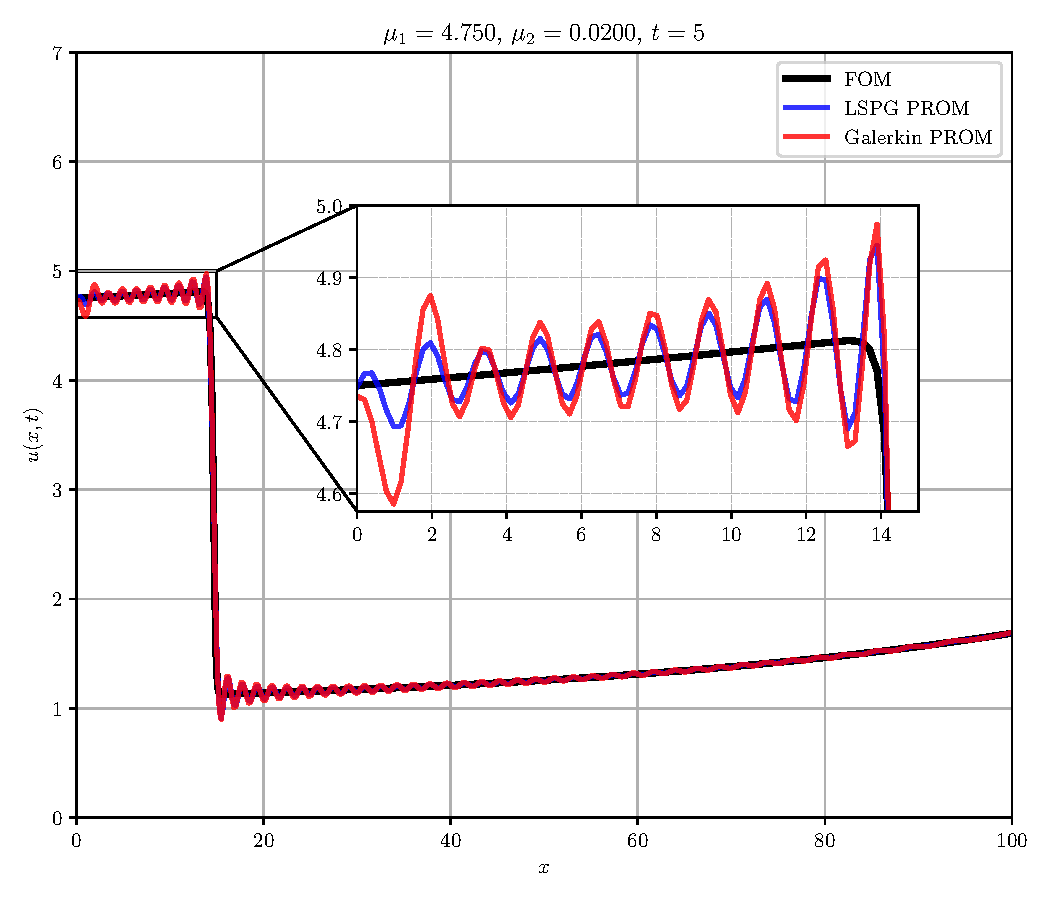
\includegraphics[width=0.7\textwidth]{Figures/fom_pod_comparison_tol_1e-04_mu1_4.750_mu2_0.0200_modes_96.pdf}
    \caption{Comparison of Galerkin and LSPG predictions at $t = 5\,\text{s}$ for $\boldsymbol{\mu} = [4.75,\, 0.0200]$, using a reduced basis with $n = 96$ modes ($\epsilon^2 = 10^{-4}$). LSPG exhibits slightly better agreement with the FOM, though both models show oscillations.}
    \label{fig:prom_comparison_test1}
\end{figure}

\section{Toward a Petrov--Galerkin framework and HPC-enabled training for industrial-scale applications}

The studies presented in this chapter underscore two complementary challenges critical for successfully applying PROMs in realistic industrial scenarios: the optimality of projection strategies and the computational efficiency required during the offline training phase.

On one hand, the one-dimensional inviscid Burgers equation, selected specifically for its nonlinear, convection-dominated character, illustrates the inherent suboptimality of classical Galerkin projection in systems governed by non-symmetric operators. While Galerkin projection is widely used in structural dynamics, where it guarantees optimality under SPD conditions, it often underperforms in computational fluid dynamics and other fields characterized by strong convection and non-symmetric operators. In such cases, Galerkin-based reduced-order models may exhibit suboptimal accuracy or even instability.

The LSPG projection offers a valuable alternative by explicitly minimizing the discrete residual norm, providing improved robustness and accuracy in these challenging regimes. However, standard LSPG implementations pose practical difficulties, particularly in the finite element setting, where evaluating residual contributions often requires a complementary mesh when applying hyper-reduction techniques such as ECM or ECSW.

Motivated by this critical limitation:
\begin{itemize}
    \item \textbf{Chapter~\ref{chap:article1}} introduces a novel Petrov--Galerkin formulation specifically developed to retain the optimal residual-minimization properties of LSPG while circumventing the necessity of using a complementary mesh. This innovative approach significantly streamlines hyper-reduced model implementation, particularly when integrated with standard finite element environments. Although this novel Petrov--Galerkin projection introduces an additional offline training phase, the associated computational overhead remains offline, and the resultant online computations achieve significant reductions in complexity, only requiring evaluations on the reduced set of elements directly selected by the hyper-reduction strategy (e.g., ECM).
\end{itemize}

On the other hand, the reduced-order modeling of the wind turbine blade served as an illustrative preamble for realistic industrial scenarios. Although simplified, this test case revealed that practical applications inherently demand extensive parametric studies, encompassing different loading conditions, material properties, geometric variations, and finer computational discretizations.
Such comprehensive explorations can quickly render offline PROM training prohibitively expensive, surpassing the capabilities of serial computational resources. Therefore, to ensure computational feasibility and scalability, it becomes imperative to leverage HPC resources during the offline training stage. Specifically, parallelized execution of parametric high-fidelity simulations, distributed computation of SVD, and scalable implementation of hyper-reduction algorithms such as ECM are essential steps toward efficiently constructing robust PROMs. Once trained, the resulting models can be readily deployed in computationally constrained edge environments, providing real-time and accurate digital twin capabilities.

Recognizing this necessity:
\begin{itemize}
    \item \textbf{Chapter~\ref{chap:article2}} presents a comprehensive HPC-enabled workflow explicitly designed for industrial-scale reduced-order modeling. This workflow seamlessly integrates parallel execution of high-fidelity simulations, distributed training through parallel SVD algorithms, and scalable hyper-reduction techniques (by introducing a partitioned version of the ECM). The practical effectiveness and computational efficiency of the developed approach are demonstrated through an industrially relevant multiphysics application involving the thermal dynamics of an electric motor. The results clearly illustrate how HPC-driven offline training facilitates the rapid and efficient creation of robust reduced-order models, enabling their successful deployment in edge and cloud environments for real-time digital twin applications.
\end{itemize}

Collectively, the subsequent chapters consolidate these two essential components: optimal residual minimization and scalable offline HPC training, into a cohesive methodological and computational framework. This combination provides a clear pathway toward robust, accurate, and computationally feasible projection-based ROM deployment in complex, industrially relevant scenarios.

% \clearpage

% \section*{Nomenclature}

% \begin{tabbing}
% \hspace{2cm} \= \kill
% $N$ \> Number of full-order degrees of freedom (DoFs) \\
% $n$ \> Number of reduced modes in the reduced-order basis \\
% $P$ \> Number of parameter samples \\
% $N_t$ \> Number of time steps per parameter \\
% $N_s$ \> Total number of snapshots, $N_s = P \times N_t$ \\
% \( N_e \) \> Number of elements in the full-order model mesh \\
% $n_e$ \> Number of elements in the hyper-reduced mesh \\
% $\boldsymbol{\Phi}$ \> Reduced-order basis (ROB) matrix \\
% $\mathbf{S}$ \> Snapshot matrix \\
% $\mathbf{U}, \boldsymbol{\Sigma}, \mathbf{V}$ \> SVD of $\mathbf{S}$: left singular vectors, singular values, right singular vectors \\
% $\mathbf{u}(t, \boldsymbol{\mu})$ \> Full-order state vector \\
% $\mathbf{\tilde{u}}(t, \boldsymbol{\mu})$ \> Reconstructed ROM solution \\
% $\mathbf{q}(t, \boldsymbol{\mu})$ \> Generalized coordinates (reduced) \\
% $\mathbf{R}(\cdot)$ \> Full-order residual \\
% $\mathbf{J}(\cdot)$ \> Full-order Jacobian \\
% $\mathbf{R}_r(\cdot)$ \> Reduced residual (Galerkin) \\
% $\mathbf{J}_r(\cdot)$ \> Reduced Jacobian (Galerkin) \\
% $\mathbf{R}_r^{\text{LSPG}}(\cdot)$ \> Reduced residual (LSPG) \\
% $\mathbf{J}_r^{\text{LSPG}}(\cdot)$ \> Reduced Jacobian (LSPG) \\
% $\epsilon^2(n)$ \> Squared POD energy loss \\
% $\mathbb{RE}_{2, \mathbf{u}}$ \> Relative error metric for solution accuracy \\
% $\widetilde{\mathcal{E}}$ \> Reduced element subset for hyper-reduction (ECM) \\
% $\xi_e$ \> Cubature weights (ECM) \\
% FOM \> Full-Order Model \\
% PROM \> Projection-based Reduced-Order Model \\
% HPROM \> Projection-based Hyper-reduced Order Model \\
% POD \> Proper Orthogonal Decomposition \\
% LSPG \> Least-Squares Petrov--Galerkin \\
% ECM \> Empirical Cubature Method \\
% SoE \> System of Equations \\
% HPC \> High-Performance Computing
% \end{tabbing}


